\documentclass[12pt,a4paper,oneside]{report}

% =========================================================================
% CSOMAGOK BEHÍVÁSA ÉS TÍPUSBEÁLLÍTÁSOK
% =========================================================================
\usepackage[utf8]{inputenc}
\usepackage[T1]{fontenc}
\usepackage[magyar]{babel}
\usepackage{geometry}
\geometry{
    a4paper,
    left=35mm,
    right=25mm,
    top=25mm,
    bottom=25mm
}

\usepackage{amsmath, amssymb, amsfonts}
\usepackage{graphicx}
\usepackage{booktabs}
\usepackage{multirow}
\usepackage{array}
\usepackage{listings}
\usepackage{xcolor}
\usepackage{hyperref}
\usepackage{caption}
\usepackage{subcaption}
\usepackage{float}
\usepackage{tabularx}
\usepackage{setspace}
\onehalfspacing % 1.5-ös sorköz az egyetemi szabályzatnak megfelelően

% TikZ és UML rajzolás
\usepackage{tikz}
\usetikzlibrary{arrows.meta, positioning, shapes.geometric, shapes.multipart, fit, calc, backgrounds}

% Színpaletta definíciók
\definecolor{codegreen}{rgb}{0,0.6,0}
\definecolor{codegray}{rgb}{0.5,0.5,0.5}
\definecolor{codepurple}{rgb}{0.58,0,0.82}
\definecolor{backcolour}{rgb}{0.97,0.97,0.97}
\definecolor{szedarkblue}{RGB}{0, 51, 102}
\definecolor{umlblue}{RGB}{230, 240, 255}
\definecolor{umldarkblue}{RGB}{30, 80, 160}
\definecolor{umlyellow}{RGB}{255, 250, 220}
\definecolor{umlgreen}{RGB}{220, 255, 220}
\definecolor{umlred}{RGB}{255, 225, 225}

\hypersetup{
    colorlinks=true,
    linkcolor=szedarkblue,
    filecolor=magenta,      
    urlcolor=cyan,
    citecolor=szedarkblue,
    pdftitle={Gráf alapú modellek alkalmazása vizuális információ feldolgozására, különös tekintettel a viselkedéselemzésre},
    pdfauthor={Szakdolgozó Hallgató}
}

\lstdefinestyle{mystyle}{
    backgroundcolor=\color{backcolour},   
    commentstyle=\color{codegreen},
    keywordstyle=\color{magenta},
    numberstyle=\tiny\color{codegray},
    stringstyle=\color{codepurple},
    basicstyle=\ttfamily\footnotesize,
    breakatwhitespace=false,         
    breaklines=true,                 
    captionpos=b,                    
    keepspaces=true,                 
    numbers=left,                    
    numbersep=5pt,                  
    showspaces=false,                
    showstringspaces=false,
    showtabs=false,                  
    tabsize=4
}
\lstset{style=mystyle}

% =========================================================================
% DOKUMENTUM KEZDETE
% =========================================================================
\begin{document}

% --- BELSŐ CÍMLAP ---
\begin{titlepage}
    \begin{center}
        \vspace*{0.5cm}
        {\LARGE \textbf{SZÉCHENYI ISTVÁN EGYETEM}}\\[0.3cm]
        {\large \textbf{GÉPÉSZMÉRNÖKI, INFORMATIKAI ÉS VILLAMOSMÉRNÖKI KAR}}\\[0.2cm]
        {\large Informatika Tanszék}\\[2.0cm]

        \includegraphics[width=0.25\textwidth]{example-image-a}\\[1.2cm]

        {\Large \textbf{SZAKDOLGOZAT 1 -- KUTATÁSI ÉS FEJLESZTÉSI TERV}}\\[0.6cm]

        {\huge \textbf{Gráf alapú modellek alkalmazása vizuális információ feldolgozására, különös tekintettel a viselkedéselemzésre}}\\[0.4cm]
        {\large \textit{Valós idejű esésdetektálás 2D pózbecsléssel, kinematikai heurisztikákkal és tér-időbeli gráfkonvolúciós hálózatokkal (ST-GCN)}}\\[2.0cm]

        \begin{minipage}{0.48\textwidth}
            \begin{flushleft} \large
                \textbf{Készítette:}\\
                Szakdolgozó Hallgató\\
                Mérnökinformatikus BSc
            \end{flushleft}
        \end{minipage}
        \hfill
        \begin{minipage}{0.48\textwidth}
            \begin{flushright} \large
                \textbf{Témavezető:}\\
                Egyetemi Adjunktus / Konzulens\\
                Tanszéki Oktató
            \end{flushright}
        \end{minipage}

        \vfill
        {\large Győr, 2026}
    \end{center}
\end{titlepage}

% --- KIVONAT / ABSZTRAKT ---
\begin{abstract}
A gépi látás és a viselkedéselemzés egyik legkritikusabb gyakorlati alkalmazási területe a váratlan emberi esések valós idejű, megbízható felismerése. A demográfiai öregedés következtében az egyedül élő idős emberek körében az elesések száma folyamatosan emelkedik, ahol a padlón töltött idő drasztikusan növeli a súlyos szövődmények kialakulásának kockázatát. Bár a piacon elérhetők hordható vészjelzők, a felhasználói feledékenység és az eszméletvesztés miatt megbízhatóságuk korlátozott. A felhőbe képeket továbbító biztonsági kamerák pedig komoly adatvédelmi és személyiségi jogi (GDPR) ellenállásba ütköznek a magánszférában.

Jelen szakdolgozati munka (Szakdolgozat 1 -- Kutatási és fejlesztési terv) egy olyan autonóm, beépített adatvédelmet (\textit{Privacy-by-Design}) célzó esésdetektáló rendszer tervezését és elméleti megalapozását mutatja be, amely monokuláris videofolyamból nyert vizuális információt elemez. A dolgozat címében szereplő gráf alapú modellezés az emberi testtartást leíró anatómiai kulcspontok térbeli és időbeli összefüggéseinek reprezentációjára utal. A tervezett rendszer feldolgozási lánca a modern mélytanulási pózbecslő modellt (YOLOv8-Pose) ötvözi geometriai-kinematikai mozgáselemzéssel és tér-időbeli gráfkonvolúciós hálózatokkal (ST-GCN). A rendszer alapelve, hogy a nyers videokockák a kulcspontok kinyerése után azonnal törlésre kerülnek a memóriából; a döntéshozatal kizárólag a 17 anatómiai kulcspont koordináta-hálózatán történik.

A kutatás első szakaszában feltárásra kerültek a valós otthoni környezetben tipikusan fellépő téves riasztási lehetőségek és peremesetek (például a képmező szélén belépő személyek csonkolt sziluettje, a konyhapult előtti munka vagy a kanapén való szándékos elterülés), amelyek kezelésére szabályalapú kinematikai szűrők kerültek kialakításra. Egy részletes telemetriai esettanulmány keretében bemutatásra kerül a segédeszközzel (járókerettel) történő eleséskor fellépő takarás problémája is, amely kísérletileg rámutat a tisztán 2D geometriai heurisztikák korlátaira, és indokolja az ST-GCN hálózatok szükségességét. A dolgozat áttekinti a prototípuson végzett eddigi feltáró tesztek tapasztalatait, részletesen elemzi a jelenlegi heurisztikák biztonsági korlátait és kameranézet-függőségét, valamint egy strukturált kutatási és kísérleti ütemtervet határoz meg a modell tanítására, a nyilvános adathalmazokon (URFD, Le2i) végzendő független validációra és a beágyazott futtatás megalapozására.
\end{abstract}

\tableofcontents

% =========================================================================
% 1. FEJEZET: BEVEZETÉS ÉS A FELADAT KITŰZÉSE
% =========================================================================
\chapter{Bevezetés és a feladat kitűzése}

\section{Társadalmi és egészségügyi kontextus}
A fejlett társadalmak egyik legjelentősebb civilizációs és szociális kihívása a lakosság korfájának folyamatos elöregedése. Az Európai Unió statisztikai hivatala (Eurostat) és a Központi Statisztikai Hivatal (KSH) demográfiai elemzései alapján 2050-re az európai lakosság közel 30\%-a 65 év feletti lesz, miközben az egyedül élő idős emberek által fenntartott egyszemélyes háztartások aránya ugrásszerűen növekszik. 

Ebben a veszélyeztetett korosztályban az önálló életvitel elvesztésének és a súlyos egészségkárosodásoknak a vezető oka a váratlan elesés:
\begin{itemize}
    \item Az Egészségügyi Világszervezet (WHO, 2021) \cite{who2021} adatai szerint a 65 év feletti lakosság 30--35\%-a, míg a 80 év felettiek több mint 40\%-a legalább egyszer elesik évente.
    \item Bár a közhiedelemmel ellentétben az eséseknek csupán mintegy 5--10\%-a vezet közvetlen csonttöréshez, a kórházi traumatológiai ellátást igénylő combnyak- és medencetörések több mint 90\%-a elesés következménye.
    \item Az elesések közvetlen orvosi ellátási költségei, valamint a tartós ápolási és rehabilitációs kiadások az Európai Unióban és az Egyesült Államokban is évi több tízmilliárd dolláros terhet rónak az egészségbiztosítási rendszerekre.
\end{itemize}

\section{Az elhúzódó földön fekvés orvosi szövődményei és a beavatkozási időablak}
A baleseti sebészetben és az intenzív terápiában jól ismert az R. Adams Cowley által leírt ,,arany óra'' (\textit{Golden Hour}) koncepciója, amely kimondja, hogy a súlyos traumát szenvedett páciensek túlélési esélyei drasztikusan lecsökkennek, ha a végleges orvosi ellátás nem kezdődik meg a sérülést követő első 60 percen belül. Az idősgyógyászati (geriátriai) szakirodalom egyértelműen bizonyítja, hogy az elesést követő klinikai kimenetelt döntően nem maga az esés mechanikai energiája, hanem a földön töltött idő hossza (\textit{time-on-floor}) határozza meg:
\begin{enumerate}
    \item \textbf{A gyors segítségnyújtás hatása:} Amennyiben az elesett személy az eseményt követő egy órán belül szakszerű segítséget kap, a tartós szövődmények és az intézményi elhelyezés kockázata minimálisra szorítható.
    \item \textbf{Az elhúzódó fekvés (\textit{long lie}) szövődményei:} Wild és munkatársai mérföldkőnek számító kutatásai \cite{wild1981}, valamint Tinetti és kutatócsoportja \cite{tinetti1993} kimutatták, hogy amennyiben egy idős ember egyedül esik el és több mint 1 órát mozdulatlanul a földön tölt, a halálozási ráta 6 hónapon belül meghaladja az 50\%-ot -- még abban az esetben is, ha közvetlen mechanikai törést nem szenvedett. Ennek hátterében a következő patofiziológiai folyamatok állnak:
    \begin{itemize}
        \item \textit{Hipotermia (kihűlés):} A hideg padlóburkolattal való közvetlen érintkezés még fűtött szobában is gyors hővesztéshez és veszélyes maghőmérséklet-csökkenéshez vezet.
        \item \textit{Rhabdomyolysis (izomelhalás):} A saját testsúly okozta tartós nyomás alatt a komprimált izomsejtek ischaemiás nekrózist szenvednek, aminek következtében nagymennyiségű mioglobin és kálium áramlik a véráramba, akut tubuláris nekrózist és veseelégtelenséget idézve elő.
        \item \textit{Dekubitusz és keringési elégtelenség:} A sokkos állapot és a mozdulatlanság órák alatt súlyos szöveti elhalást és keringési összeomlást okoz.
    \end{itemize}
\end{enumerate}

\section{Meglévő technológiai megközelítések és korlátaik}
Az elesések automatizált detektálására az elmúlt évtizedben számos mérnöki megoldás született, ezek azonban a gyakorlatban komoly korlátokba ütköznek:

\begin{table}[H]
\centering
\small
\begin{tabularx}{\textwidth}{p{3.0cm}p{3.2cm}Xp{3.8cm}}
\toprule
\textbf{Megközelítés típusa} & \textbf{Tipikus megvalósítások} & \textbf{Főbb előnyök} & \textbf{Gyakorlati korlátok és hátrányok} \\
\midrule
\textbf{Hordható eszközök (Wearables)} & Gyorsulásmérős (IMU) okosórák, medálok, segélyhívó gombok \cite{kwolek2014} & Olcsó, testen hordozható, kültéren is működik & Felhasználói feledékenység (az idősek fürdéskor, alváskor leveszik). Eszméletvesztésnél a pánikgomb nem nyomható meg. \\
\midrule
\textbf{Környezeti szenzorok} & Intelligens padlószőnyeg, Doppler-radar, akusztikus mikrofonhálózat & Nem kell viselni, nem sérti a képi magánszférát & Bonyolult és drága telepítés, szobánkénti kalibráció, nem nyújt részletes vizuális információt a mozgás típusáról. \\
\midrule
\textbf{Hagyományos biztonsági kamerák} & Felhőbe streamelő beltéri IP kamerák, nyers képanalízis \cite{rougier2011} & Gazdag vizuális információ, nagy látószög & \textbf{Súlyos etikai és adatvédelmi (GDPR) ellenállás:} A magánélet legintimebb tereiben (hálószoba, fürdőszoba) a videostreaming elfogadhatatlan. \\
\midrule
\textbf{Beépített adatvédelmű gépi látás (Jelen munka)} & Helyi pózbecslés (YOLOv8-Pose) + Gráf- és kinematikai analízis & Nincs hordható eszköz, a nyers képkockák azonnal megsemmisülnek, valós idejű & Komplex algoritmust és modellezést igényel a peremesetek, takarások és szándékos leülések kezelésére. \\
\bottomrule
\end{tabularx}
\caption{Az esésdetektálási technológiák összehasonlító elemzése.}
\label{tab:tech_comparison}
\end{table}

\section{A szakdolgozat célkitűzései és a tervezett rendszer áttekintése}
A szakdolgozat átfogó mérnöki célkitűzése egy olyan autonóm, monokuláris kameraképre épülő esésdetektáló szoftverrendszer megtervezése és megvalósítása, amely képes a lakókörnyezetben bekövetkező hirtelen mozgásvesztéseket megbízhatóan felismerni, miközben maximálisan tiszteletben tartja a felhasználók személyiségi jogait és magánszféráját. 

A munka a következő főbb pillérekre épül:
\begin{enumerate}
    \item \textbf{Beépített adatvédelem (Privacy-by-Design):} A nyers videokockák feldolgozása kizárólag a helyi számítási egység memóriájában történik. A 2D kulcspontok kinyerése után a képi információ azonnal törlésre kerül, így sem képi, sem videós adatfolyam nem hagyja el a helyi eszközt, és semmilyen vizuális tartalom nem kerül tartós tárolásra.
    \item \textbf{Kétrétegű detektálási architektúra:}
    \begin{itemize}
        \item \textit{Elsődleges gyors kinematikai szűrő:} Egy valós idejű, szabályalapú állapotgép (FSM), amely a testtartás arányaiból, a gerincvektor dőlésszögéből és a súlypont vertikális sebességéből szűri a mindennapi életviteli tevékenységeket (ADL).
        \item \textit{Tér-időbeli gráfkonvolúciós hálózat (ST-GCN):} A csontváz-topológia időbeli dinamikáját modellező mélytanulási réteg beépítése, amely a takarások és összetett dinamikus átmenetek esetén is képes a mozgásmintázat helyes osztályozására.
    \end{itemize}
    \item \textbf{Robusztus peremeset-kezelés:} Olyan algoritmikus mechanizmusok kifejlesztése, amelyek megakadályozzák a valós háztartási környezetben tipikusan fellépő téves riasztásokat (például a képmező szélén belépő személyek csonkolt bounding boxai, a konyhapult előtti munka vagy a kanapén való szándékos elterülés).
    \item \textbf{Erőforrás-hatékony futtatás:} A teljes feldolgozási lánc optimalizálása annak érdekében, hogy költséges, dedikált nagy teljesítményű GPU hardver nélkül, átlagos asztali számítógépen vagy laptop processzoron (CPU) is biztosítható legyen a valós idejű (folyamatos, legalább 25 FPS képkockasebességű) működés, valamint a jövőbeni beágyazott (pl. Raspberry Pi alapú) futtatás megalapozása.
\end{enumerate}

\section{Kutatási kérdések és hipotézisek}
A kutatómunka és a tervezési folyamat irányítására a következő tudományos kutatási kérdések (\textit{Research Questions - RQ}) és formális hipotézisek (\textit{Hypotheses - H}) kerültek megfogalmazásra:
\begin{itemize}
    \item \textbf{RQ1:} Képes-e a monokuláris 2D emberi pózbecslés mélységszenzor (RGB-D) nélkül, tisztán geometriai és kinematikai idősorok alapján megbízhatóan szétválasztani a mindennapi életviteli mozgásokat (ADL) a valódi esésektől?
    \begin{itemize}
        \item \textbf{H1:} A normalizált bounding box képarány ($AR$), a gerincvektor dőlésszöge ($\theta_{\text{torso}}$) és a súlypont vertikális sebességének ($v_y$) együttes állapotgépes modellezésével a tipikus leülések és tárgyért hajolások szignifikánsan elkülöníthetők az esési tranziensektől.
    \end{itemize}
    \item \textbf{RQ2:} Milyen mértékben torzítja a segédeszközök (pl. járókeret) általi részleges kitakarás a detektált kulcspontok folytonosságát, és kompenzálható-e ez a jelenség tisztán 2D geometriai szinten?
    \begin{itemize}
        \item \textbf{H2:} A talajszinthez közeli fizikai takarások a kulcspontok hirtelen elvesztéséhez és az észlelt sziluett ugrásszerű zsugorodásához vezetnek, amely hagyományos heurisztikákkal csak esési előzménymemória bevonásával kezelhető, végső megoldása pedig a csontváz-gráf összefüggéseit tanuló tér-időbeli modellezést (ST-GCN) igényli.
    \end{itemize}
    \item \textbf{RQ3:} Milyen feltételek mellett képes egy térbeli képsíki szintmodell megkülönböztetni a bútoron (ágyon, kanapén) történő pihenést a padlóra zuhanástól?
    \begin{itemize}
        \item \textbf{H3:} Rögzített látószögű kameránál a padlózóna alsó képtartományának küszöbölése és a sebességcsillapodás szűri a kanapén való elterülést, azonban a távoli háttérben bekövetkező eséseknél hamis negatív döntést eredményezhet, ami a kamera geometriai kalibrációját vagy tanult térbeli reprezentációt tesz szükségessé.
    \end{itemize}
    \item \textbf{RQ4:} Megvalósítható-e a teljes feldolgozási lánc (pózbecslés, geometriai elemzés, állapotgép és megjelenítés) valós időben ($\ge 25$ FPS képkockasebességgel) átlagos felhasználói számítógépen, dedikált nagy teljesítményű grafikus gyorsító (GPU) nélkül, tisztán CPU-n futtatva?
    \begin{itemize}
        \item \textbf{H4:} A könnyített architektúrájú mélytanuló modellek (YOLOv8n-Pose / YOLOv8s-Pose) és a vektorizált kinematikai számítások ciklusideje optimalizált futtatókörnyezetben átlagos asztali számítógép processzorán 40 ms alatt tartható, biztosítva a 25 FPS feletti folyamatos feldolgozást.
    \end{itemize}
\end{itemize}

% =========================================================================
% 2. FEJEZET: SZAKIRODALMI ÁTTEKINTÉS ÉS ELMÉLETI HÁTTÉR
% =========================================================================
\chapter{Szakirodalmi áttekintés és elméleti háttér}

A számítógépes látással és mélytanulással megvalósított emberi viselkedéselemzés és esésdetektálás az elmúlt évtizedben jelentős paradigmaváltáson ment keresztül. A korai, tisztán sziluett- és optikai áramlás (\textit{optical flow}) alapú módszereket felváltották az anatómiai kulcspontokat becslő konvolúciós architektúrák, valamint az emberi vázat tér-időbeli gráfként reprezentáló mély hálózatok. Jelen fejezet bemutatja a tervezett rendszer elméleti és matematikai alapjait: a 2D mélytanulási pózbecslést, a származtatott kinematikai mozgásjellemzőket, a tér-időbeli gráfkonvolúciós hálózatok (ST-GCN) működését, az adatvédelmi (\textit{Privacy-by-Design}) szempontok mérnöki realitását, valamint a kapcsolódó nemzetközi szakirodalom kritikai összehasonlítását.

\section{Emberi pózbecslés mélytanulással}
Az emberi testtartás képi rekonstrukciója (2D Human Pose Estimation) a számítógépes látás egyik legintenzívebben kutatott területe. A cél az emberi test anatómiailag releváns ízületeinek és végtagpontjainak képsíki lokalizációja egyetlen RGB képkocka alapján.

\subsection{A pózbecslő architektúrák evolúciója}
A szakirodalomban a pózbecslési megközelítések alapvetően két fő csoportra oszthatók:
\begin{enumerate}
    \item \textbf{Felülről lefelé építkező (Top-down) módszerek:} Első lépésben egy emberdetektáló modell behatárolja az egyéneket reprezentáló befoglaló téglalapokat (\textit{bounding box}), majd egy specializált hálózat (pl. AlphaPose, HRNet) minden egyes kivágott területen külön megbecsüli a kulcspontok hőtérképeit (\textit{heatmaps}). Bár ezen modellek pontossága kiemelkedő, számítási igényük lineárisan skálázódik a képen látható személyek számával, ami jelentős késleltetést okoz.
    \item \textbf{Alulról felfelé építkező (Bottom-up) módszerek:} A teljes képen egyszerre detektálják az összes létező kulcspontot, majd asszociációs mezők (pl. az OpenPose által bevezetett \textit{Part Affinity Fields}, PAF \cite{cao2019openpose}) segítségével kapcsolják össze az egymáshoz tartozó ízületeket. Számítási idejük független a személyek számától, azonban a hőtérképek pixel-szintű dekódolása számításigényes utófeldolgozást igényel.
\end{enumerate}

A valós idejű, erőforrás-korlátos működés megvalósításához a legkorszerűbb \textbf{egyfokozatú, horgonypont-mentes (Single-stage, Anchor-free)} architektúrák kínálják az optimális kompromisszumot. Jelen kutatásban az Ultralytics cég \textbf{YOLOv8-Pose} \cite{yolov8pose} architektúrája kerül alkalmazásra:
\begin{itemize}
    \item \textit{Gerinchálózat (Backbone):} Módosított CSPDarknet, amely C2f blokkokat alkalmaz a gazdag kontextus kinyerésére alacsony számítási költség mellett.
    \item \textit{Nyakrész (Neck):} Továbbfejlesztett PANet (Path Aggregation Network), amely piramisszerűen ötvözi a többskálájú térbeli információkat.
    \item \textit{Detektáló és regressziós fej (Head):} Szétválasztott (\textit{decoupled}) kimeneti rétegek, ahol a befoglaló téglalap osztályozása mellett egy közvetlen regressziós ág becsli meg a kulcspontok koordinátáit és láthatósági valószínűségeit.
\end{itemize}

\subsection{A COCO-17 topológia és az OKS veszteségfüggvény}
A modell a nemzetközileg standardizált MS COCO topológiát \cite{coco2014} követi, amely az emberi testet $N = 17$ diszkrét kulcsponttal írja le. Minden egyes személy pózreprezentációja egy $K$ halmazként értelmezhető:
\begin{equation}
    K = \left\{ \mathbf{p}_i = (x_i, y_i, c_i) \right\}_{i=1}^{17}
\end{equation}
ahol $(x_i, y_i) \in \mathbb{R}^2$ a kulcspont normalizált képsíki koordinátái, $c_i \in [0, 1]$ pedig a hálózat által predikált konfidencia-érték.

A kulcspont-regresszió tanítási folyamatának alapját az \textbf{OKS (Object Keypoint Similarity)} metrika képezi:
\begin{equation}
    OKS = \frac{\sum_{i=1}^{17} \exp\left( - \frac{d_i^2}{2 s^2 \sigma_i^2} \right) \delta(v_i > 0)}{\sum_{i=1}^{17} \delta(v_i > 0)}
\end{equation}
ahol $d_i = \|\mathbf{p}_i - \hat{\mathbf{p}}_i\|_2$ a becsült és valós kulcspont euklideszi távolsága, $s = \sqrt{W \cdot H}$ a személy méretskálája, $\sigma_i$ az adott kulcspont anatómiai varianciája (orr/szem: $\sigma \approx 0{,}025-0{,}035$, csípő/boka: $\sigma \approx 0{,}087-0{,}107$), $v_i$ a láthatósági indikátor, $\delta(\cdot)$ pedig a feltételes indikátorfüggvény. A kulcspontok esésanalízisbeli szerepét a \ref{tab:coco_keypoints}. táblázat részletezi.

\begin{table}[H]
\centering
\small
\begin{tabularx}{\textwidth}{cllX}
\toprule
\textbf{Index ($i$)} & \textbf{Kulcspont megnevezése} & \textbf{Anatómiai régió} & \textbf{Szerepe és fontossága az eséselemzésben} \\
\midrule
\textbf{0} & Orr (\textit{Nose}) & Fej & A hirtelen lefelé irányuló mozgástranziens (zuhanás) legfelső indikátora. \\
\textbf{1, 2} & Szemek (\textit{Left/Right Eye}) & Fej & A fej térbeli orientációjának és forgatásának becslése. \\
\textbf{3, 4} & Fülek (\textit{Left/Right Ear}) & Fej & A fej laterális billenésének és a fejtartás elvesztésének azonosítása. \\
\textbf{5, 6} & Vállak (\textit{Left/Right Shoulder}) & Felsőtest & A gerincvektor felső rögzítési pontja; a vállszélesség a testméret referenciája. \\
\textbf{7, 8} & Könyökök (\textit{Left/Right Elbow}) & Felső végtagok & Védekező reflexmozdulatok és kitámasztási kísérletek vizsgálata. \\
\textbf{9, 10} & Csuklók (\textit{Left/Right Wrist}) & Felső végtagok & Talajjal való érintkezés, tompítás és magatehetetlenség elemzése. \\
\textbf{11, 12} & Csípők (\textit{Left/Right Hip}) & Medence & \textbf{A test tömegközéppontjának (CoM) és a gerinc alsó pontjának alapja.} \\
\textbf{13, 14} & Térdek (\textit{Left/Right Knee}) & Alsó végtagok & Térdhajlítás mérése, a leülés és leguggolás szétválasztása az eséstől. \\
\textbf{15, 16} & Bokák (\textit{Left/Right Ankle}) & Alsó végtagok & A talajsík fizikai érintési zónája; a vízszintes kiterjedés ellenőrzése. \\
\bottomrule
\end{tabularx}
\caption{A COCO-17 kulcspont-topológia anatómiai szerepe az eséselemzésben.}
\label{tab:coco_keypoints}
\end{table}

\section{Kinematikai mozgásjellemzők és paraméterhierarchia}
A kulcspontok koordinátáiból származtatott differenciális és szögjellemzők képezik az állapotgép bemenetét.

\subsection{Befoglaló téglalap és képarány}
A detektált kulcspontok kiterjedése alapján meghatározható a személyt körülvevő téglalap ($W = \max(1{,}0, x_2 - x_1)$, $H = \max(1{,}0, y_2 - y_1)$), amelyből a képarány ($AR$):
\begin{equation}
    AR = \frac{W}{H}
\end{equation}

\subsection{A törzs dőlésszögei (Roll és Sagittal Pitch)}
A vállak ($\mathbf{p}_{\text{váll}} = \frac{\mathbf{p}_5 + \mathbf{p}_6}{2}$) és csípők ($\mathbf{p}_{\text{csípő}} = \frac{\mathbf{p}_{11} + \mathbf{p}_{12}}{2}$) felezőpontjaiból számított gerincvektor frontális dőlésszöge:
\begin{equation}
    \theta_{\text{roll}} = \arctan\left( \frac{|x_{\text{váll}} - x_{\text{csípő}}|}{|y_{\text{váll}} - y_{\text{csípő}}| + \epsilon} \right) \cdot \frac{180^\circ}{\pi}
\end{equation}
A szagittális (kamera felé vagy attól távolodó) dőlés a törzs magassági arányából ($\text{torso\_ratio} = \frac{|y_{\text{váll}} - y_{\text{csípő}}|}{H}$) becsülhető, szigorúan levágva a negatív tartományt:
\begin{equation}
    \theta_{\text{pitch}} = \max\left( 0{,}0^\circ, \min\left( 80{,}0^\circ, \frac{0{,}16 - \text{torso\_ratio}}{0{,}12} \cdot 60{,}0^\circ \right) \right)
\end{equation}
A test teljes dőlésszöge a két komponens maximuma:
\begin{equation}
    \theta_{\text{torso}} = \max(\theta_{\text{roll}}, \theta_{\text{pitch}})
\end{equation}

\subsection{A tömegközéppont vertikális sebessége}
A csípőpontok felezőpontjából számított normalizált vertikális sebesség ($\text{ref\_size} = \max(W, H, 50{,}0)$):
\begin{equation}
    v_y(t) = \frac{y_{\text{CoM}}(t) - y_{\text{CoM}}(t - \Delta t)}{\Delta t \cdot \text{ref\_size}}
\end{equation}

\subsection{Paraméterhierarchia}
A döntési állapotgépben alkalmazott paraméterek fizikai szerepét a \ref{tab:param_hierarchy}. táblázat rendszerezi.

\begin{table}[H]
\centering
\small
\begin{tabularx}{\textwidth}{p{2.2cm}cp{2.2cm}X}
\toprule
\textbf{Paraméter} & \textbf{Küszöb} & \textbf{Mértékegység} & \textbf{Állapotgépes szerep és mérnöki indoklás} \\
\midrule
$v_{y,\text{drop}}$ & $> 0{,}45$ & $\text{frame}^{-1}$ & \textbf{Kritikus zuhanás (Drop detected):} Extrém gyors vertikális zuhanási fázis. \\
$v_{y,\text{fast}}$ & $> 0{,}35$ & $\text{frame}^{-1}$ & \textbf{Gyors esési tranziens:} Megerősíti az aktív dőlési mozgást ($FALLING$ állapot). \\
$v_{y,\text{warn}}$ & $> 0{,}22$ & $\text{frame}^{-1}$ & \textbf{Előzetes figyelmeztetés:} Alacsonyabb sebességküszöb mérsékelt dőlés esetén. \\
$v_{y,\text{rest}}$ & $|v_y| < 0{,}28$ & $\text{frame}^{-1}$ & \textbf{Mozgási stabilizáció:} Nyugalmi ablak bútoron történő ülés/fekvés igazolására. \\
$v_{y,\text{counter}}$ & $< 0{,}25$ & $\text{frame}^{-1}$ & \textbf{Konyhapult plafon:} Maximális mozgásingadozás felállás/munka közben. \\
$AR_{\text{floor}}$ & $> 1{,}15$ & dimenziótlan & \textbf{Padlószinti fekvés:} Szigorú fekvő testhelyzet küszöb a talajzónában. \\
$AR_{\text{rest}}$ & $> 0{,}95$ & dimenziótlan & \textbf{Bútorszinti pihenés:} Enyhített arány bútoron való elnyúlás kezelésére. \\
$\theta_{\text{fall}}$ & $> 45{,}0^\circ$ & fok ($^\circ$) & \textbf{Esési dőlésszög:} Határérték, amely felett a gerinc horizontális. \\
$\theta_{\text{rest}}$ & $> 28{,}0^\circ$ & fok ($^\circ$) & \textbf{Pihenési dőlésszög:} Enyhébb szögküszöb ülő/dőlt bútorpozíció detektálására. \\
$y_{2,\text{floor}}$ & $\ge 0{,}70 \cdot H$ & képmagasság & \textbf{Padlózóna heurisztika:} Feltételezi, hogy a padló a kép alsó 30\%-ában van. \\
$N_{\text{mem}}$ & $12$ képkocka & $\approx 0{,}48$ s & \textbf{Zuhanási előzménymemória:} Időablak a zuhanás utáni takarások áthidalására. \\
\bottomrule
\end{tabularx}
\caption{A döntési állapotgép szintezett paraméterhierarchiája.}
\label{tab:param_hierarchy}
\end{table}

\section{Tér-időbeli Gráfkonvolúciós Hálózatok (ST-GCN) elmélete}
A szabályalapú állapotgépek korlátait a csontváz-topológia közvetlen modellezésével az ST-GCN \cite{yan2018stgcn} hálózatok oldják fel.

\subsection{Tér-időbeli gráf reprezentáció}
Az emberi testmozgást egy $G = (V, E)$ irányítatlan gráf reprezentálja, ahol $V = \{ v_{ti} \mid t = 1, \dots, T; i = 1, \dots, N \}$ a csúcsok halmaza ($N = 17$, $T = 30-60$). Az élek halmaza két komponenst tartalmaz:
\begin{enumerate}
    \item \textbf{Intra-frame térbeli élek ($E_S$):} Természetes biológiai ízületi kapcsolatok egy adott képkockán belül.
    \item \textbf{Inter-frame időbeli élek ($E_T$):} Az azonos anatómiai pontok időbeli pályáját összekötő élek ($v_{ti} \to v_{(t+1)i}$).
\end{enumerate}

\begin{figure}[H]
\centering
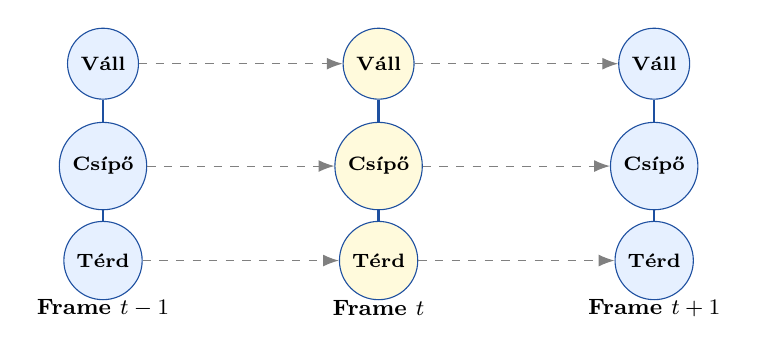
\begin{tikzpicture}[
    joint/.style={circle, draw=umldarkblue, fill=umlblue, minimum size=6mm, font=\scriptsize\bfseries},
    timeedge/.style={draw=gray, dashed, -{Latex[length=2mm]}},
    spatedge/.style={draw=umldarkblue, thick}
]
    \node[joint] (s1) at (0, 2.5) {Váll};
    \node[joint] (h1) at (0, 1.2) {Csípő};
    \node[joint] (k1) at (0, 0) {Térd};
    \draw[spatedge] (s1) -- (h1);
    \draw[spatedge] (h1) -- (k1);
    \node[font=\footnotesize\bfseries] at (0, -0.6) {Frame $t-1$};

    \node[joint, fill=umlyellow] (s2) at (3.5, 2.5) {Váll};
    \node[joint, fill=umlyellow] (h2) at (3.5, 1.2) {Csípő};
    \node[joint, fill=umlyellow] (k2) at (3.5, 0) {Térd};
    \draw[spatedge] (s2) -- (h2);
    \draw[spatedge] (h2) -- (k2);
    \node[font=\footnotesize\bfseries] at (3.5, -0.6) {Frame $t$};

    \node[joint] (s3) at (7, 2.5) {Váll};
    \node[joint] (h3) at (7, 1.2) {Csípő};
    \node[joint] (k3) at (7, 0) {Térd};
    \draw[spatedge] (s3) -- (h3);
    \draw[spatedge] (h3) -- (k3);
    \node[font=\footnotesize\bfseries] at (7, -0.6) {Frame $t+1$};

    \draw[timeedge] (s1) -- (s2);
    \draw[timeedge] (s2) -- (s3);
    \draw[timeedge] (h1) -- (h2);
    \draw[timeedge] (h2) -- (h3);
    \draw[timeedge] (k1) -- (k2);
    \draw[timeedge] (k2) -- (k3);
\end{tikzpicture}
\caption{A tér-időbeli vázgráf (ST-GCN) topológiája és élkapcsolatai.}
\label{fig:stgcn_topology}
\end{figure}

\subsection{A térbeli gráfkonvolúciós operátor és partíciók}
A gráfkonvolúciós művelet:
\begin{equation}
    f_{\text{out}}(v_{ti}) = \sum_{v_{tj} \in B(v_{ti})} \frac{1}{Z_{ti}(v_{tj})} f_{\text{in}}(v_{tj}) \cdot \mathbf{w}\left(l_{ti}(v_{tj})\right)
\end{equation}
ahol $B(v_{ti})$ az 1-szomszédság, $Z$ a normalizáló együttható, $\mathbf{w}$ a tanulható súlyfüggvény. A térbeli konfigurációs partíció három diszkrét csoportot képez: gyökérpont ($l=0$), centripetális szomszédok a súlyponthoz közelebb ($l=1$), és centrifugális szomszédok ($l=2$). Mátrix formában dinamikus figyelem-maszkkal ($\mathbf{M}_k$):
\begin{equation}
    \mathbf{F}_{\text{out}} = \sum_{k=0}^{K_v - 1} \mathbf{\Lambda}_k^{-\frac{1}{2}} \left( \mathbf{A}_k \odot \mathbf{M}_k \right) \mathbf{\Lambda}_k^{-\frac{1}{2}} \mathbf{F}_{\text{in}} \mathbf{W}_k
\end{equation}

\section{Privacy-by-Design adatvédelem a mérnöki valóság tükrében}
A rendszer az EU GDPR 9. cikkének \cite{gdpr2016} megfelelve a \textit{Privacy-by-Design} (25. cikk) elvet követi:
\begin{enumerate}
    \item \textbf{Lokális illékony pufferelés:} A kamerakép kizárólag a helyi számítási egység memóriájában él.
    \item \textbf{Azonnali megsemmisítés:} A kulcspontok kinyerése után a képkockák memóriaterülete azonnal felszabadul; semmilyen képi adat nem tárolódik vagy kerül hálózatra.
    \item \textbf{Koordináta-alapú döntés:} A teljes döntési lánc lebegőpontos koordinátákon fut.
\end{enumerate}

Azonban mérnöki szempontból rá kell mutatni a Python futtatókörnyezet korlátaira:
\begin{itemize}
    \item A Python automatikus szemétgyűjtője (GC) miatt a fizikai memóriafelülírás nem azonnali; adatreziduumok maradhatnak a RAM-ban.
    \item A csontváz-idősorok egyedi mozgásmintázata puha-biometrikus (\textit{soft-biometrics}) azonosításra adhat lehetőséget.
    \item Végleges orvosi alkalmazásban ezért a C++ nyelvű megvalósítás, a titkosított RAM-bufferek és hardveres memóriatörlési függvények elengedhetetlenek.
\end{itemize}

\section{Kapcsolódó munkák és szakirodalmi összehasonlítás (Related Work)}
A számítógépes látáson alapuló esésdetektálás technológiai irányait és eredményeit a \ref{tab:related_work}. táblázat hasonlítja össze.

\begin{table}[H]
\centering
\small
\begin{tabularx}{\textwidth}{p{3.2cm}p{2.2cm}p{2.8cm}p{2.8cm}X}
\toprule
\textbf{Megközelítés} & \textbf{Bemenet} & \textbf{Osztályozó} & \textbf{Eredmény / Metrika} & \textbf{Fő korlátok} \\
\midrule
Rougier et al. (2011) \cite{rougier2011} & Monokuláris RGB & 3D fejtrajektória heurisztika & Szenzitivitás: ~90\% (Le2i) & Fényváltozásra és árnyékokra érzékeny. \\
Foroughi et al. (2008) \cite{foroughi2008} & Monokuláris RGB & Sajáttér alakjellemzők + SVM & Szenzitivitás: ~88\% & Mozgó háttértárgyakra instabil. \\
Kwolek \& Kepski (2014) \cite{kwolek2014} & RGB-D + IMU & SVM és k-NN & F1-score: ~96\% (URFD) & Drága hardver, infravörös zavarérzékenység. \\
Cao et al. (2019) / OpenPose \cite{cao2019openpose} & Monokuláris RGB & Többrétegű LSTM & F1-score: ~93\% (Le2i) & Magas számításigény (GPU szükséges). \\
Yan et al. (2018) / ST-GCN \cite{yan2018stgcn} & Csontváz-gráf & Tér-időbeli konvolúció & Pontosság: >90\% (NTU-RGB+D) & Erőforrás-igényes, asztali GPU-ra tervezett. \\
\midrule
\textbf{Jelen kutatási terv} & Monokuláris RGB & \textbf{Hibrid Kinematikai FSM + ST-GCN} & \textbf{Cél: F1 > 95\% (URFD, Le2i)} & \textbf{Alacsony költség, Privacy-by-Design, CPU-optimalizált} \\
\bottomrule
\end{tabularx}
\caption{Képi esésdetektálási módszerek összehasonlító elemzése a szakirodalomban.}
\label{tab:related_work}
\end{table}

% =========================================================================
% 3. FEJEZET: RENDSZERTERVEZÉS ÉS SZOFTVERARCHITEKTÚRA
% =========================================================================
\chapter{Rendszertervezés és Szoftverarchitektúra}

Egy autonóm, beágyazott adatvédelmet megvalósító biztonságtechnikai rendszer fejlesztése szigorú szoftvertervezési módszertant igényel. A rendszernek egyszerre kell megfelelnie a valós idejű futási kényszereknek, a minimális téves riasztási aránynak, valamint a szigorú adatvédelmi előírásoknak. Jelen fejezet bemutatja a rendszer funkcionális és nem-funkcionális követelményspecifikációját, a moduláris csővezeték-architektúrát (\textit{Pipe-and-Filter}), a részletes UML osztály- és szekvenciaterveket, a kinematikai állapotgép formális specifikációját, valamint a tervezett hibrid (kinematikai FSM + ST-GCN) döntési mechanizmus integrációs felületét.

\section{Követelményspecifikáció}

\subsection{Funkcionális követelmények (FR)}
A funkcionális követelmények a rendszer által kötelezően nyújtandó szolgáltatásokat rögzítik a \ref{tab:functional_reqs}. táblázat szerint.

\begin{table}[H]
\centering
\small
\begin{tabularx}{\textwidth}{lp{3.5cm}X}
\toprule
\textbf{Azonosító} & \textbf{Megnevezés} & \textbf{Részletes mérnöki leírás és működés} \\
\midrule
\textbf{FR-01} & Videofolyam fogadása & Monokuláris videofolyam fogadása élő USB/UVC webkameráról, RTSP IP-hálózati kamerastreamből, valamint offline tesztvideókból (.mp4, .avi). \\
\textbf{FR-02} & 2D emberi pózbecslés & Képkockánként detektálja a személyeket, regresszálva a COCO-17 topológiájú 17 kulcspont koordinátáit és konfidenciáit. \\
\textbf{FR-03} & Azonnali képmegsemmisítés & A kulcspontok kinyerése után a nyers képi puffer azonnal törlődik a memóriából (\textit{Privacy-by-Design}). \\
\textbf{FR-04} & Kinematikai elemzés & Számítja a képarányt ($AR$), a frontális dőlésszöget ($\theta_{\text{roll}}$), a szagittális dőlésszöget ($\theta_{\text{pitch}}$) és a süllyedési sebességet ($v_y$). \\
\textbf{FR-05} & Peremesetszűrés & Szűri a kép szélén belépő személyek csonkolt sziluettjét és a konyhapult előtti munkavégzést. \\
\textbf{FR-06} & Térbeli szintmodell & Megkülönbözteti a bútoron történő pihenést a padlószinti eleséstől a padlóhatárvonal és sebességstabilitás alapján. \\
\textbf{FR-07} & Állapotgépes esésdöntés & Determinisztikus állapotgép (FSM) követi a mozgás fázisait és kezeli a zuhanási memóriát. \\
\textbf{FR-08} & Tér-időbeli gráfkonvolúció & $T=30$ képkockás csúszóablakon lebegőpontos tenzorként reprezentálja a vázgráfot mély ST-GCN osztályozáshoz. \\
\textbf{FR-09} & Telemetria és riasztás & Esés igazolásakor strukturált JSON telemetriai adatcsomagot állít elő és helyi hangjelzést/értesítést indít. \\
\textbf{FR-10} & Vizuális kezelőfelület & Fejlesztői grafikus felületet (GUI) biztosít, ahol a kulcspont-váz, az állapotgép fázisa és a metrikák valós időben követhetők. \\
\bottomrule
\end{tabularx}
\caption{A tervezett rendszer funkcionális követelményei (Functional Requirements).}
\label{tab:functional_reqs}
\end{table}

\subsection{Nem-funkcionális követelmények (NFR)}
A nem-funkcionális követelmények a minőségi és teljesítménybeli peremfeltételeket írják elő a \ref{tab:non_functional_reqs}. táblázat szerint.

\begin{table}[H]
\centering
\small
\begin{tabularx}{\textwidth}{llcX}
\toprule
\textbf{Azonosító} & \textbf{Kategória} & \textbf{Mérőszám / Célérték} & \textbf{Mérnöki verifikáció módja} \\
\midrule
\textbf{NFR-01} & Futási sebesség & $\ge 25$ FPS (Ciklusidő $\le 40{,}0$ ms) & Átlagos számítógépen, GPU nélkül, tisztán CPU-n mérve. \\
\textbf{NFR-02} & Észlelési késleltetés & $T_{\text{latency}} \le 1{,}0$ másodperc & $T_{\text{latency}} = T_{\text{detect}} - T_{\text{impact}}$ (földre érkezéshez képest). \\
\textbf{NFR-03} & Szenzitivitás & $TPR \ge 95{,}0\%$ teszthalmazon & Teljes URFD és Le2i független benchmark adatbázisokon. \\
\textbf{NFR-04} & Téves riasztási arány & $FPR \le 5{,}0\%$ normál életvitelnél & Hosszú idejű ADL videókon (leülés, hajolás, fekvés). \\
\textbf{NFR-05} & Adatvédelem & $0$ képi bájt tartós tárolása & Memória-inspekcióval igazolt Privacy-by-Design. \\
\textbf{NFR-06} & Erőforrás-igény & RAM $\le 600$ MB & Beágyazott profilozás (Raspberry Pi felkészítés). \\
\textbf{NFR-07} & Hordozhatóság & Platformfüggetlen Python/ONNX & Windows, x86-64 Linux és ARM64 Linux támogatás. \\
\bottomrule
\end{tabularx}
\caption{A tervezett rendszer nem-funkcionális követelményei (Non-Functional Requirements).}
\label{tab:non_functional_reqs}
\end{table}

\section{Szoftverarchitektúra és csővezeték-modell}
A feldolgozási lánc a \textit{Pipe-and-Filter} tervezési mintát követi, amely szigorúan szétválasztja az egyes szinteket:
\begin{enumerate}
    \item \textbf{Bemeneti réteg (Video Ingestion):} Nyers képkockák folyamatos beolvasása egy illékony memóriapufferbe (\texttt{FrameBuffer}).
    \item \textbf{Pózbecslő réteg (YOLOv8-Pose):} COCO-17 koordináták regressziója, amit a nyers forráskép memóriából való azonnali felszabadítása követ.
    \item \textbf{Kinematikai és térbeli szűrőréteg:} Skálainvariáns metrikák ($AR, \theta, v_y$) számítása, szélső belépés és konyhapult-védelem.
    \item \textbf{Hibrid döntési réteg:} Determinisztikus véges állapotgép (FSM) és $T=30$ csúszóablakon futó ST-GCN mélytanuló modell döntési arbitrációja.
    \item \textbf{Kimeneti réteg:} Riasztások szétküldése (\texttt{AlertDispatcher}) és valós idejű telemetria kirajzolása (\texttt{GUIController}).
\end{enumerate}

\section{UML Rendszertervezés}
A rendszer objektumorientált osztálystruktúráját és kapcsolatait a \ref{fig:uml_detailed_class}. ábra részletezi.

\begin{figure}[H]
\centering
\begin{tikzpicture}[
    class/.style={rectangle, draw=umldarkblue, fill=umlblue, rounded corners, minimum width=3.6cm, font=\tiny, inner sep=3pt},
    line/.style={draw=umldarkblue, -{Latex[length=2.0mm]}, thick}
]
    \node[class] (video) at (0, 0) {
        \textbf{VideoSource}\\
        \hline
        - source\_path: str\\
        - cap: cv2.VideoCapture\\
        - fps: float\\
        \hline
        + open(): bool\\
        + read\_frame(): ndarray\\
        + release(): void
    };

    \node[class] (fb) at (4.2, 0) {
        \textbf{FrameBuffer}\\
        \hline
        - current\_frame: ndarray\\
        - timestamp: float\\
        \hline
        + set\_frame(f): void\\
        + purge(): void
    };

    \node[class] (yolo) at (8.4, 0) {
        \textbf{YOLOv8PoseEstimator}\\
        \hline
        - model: YOLO\\
        - conf\_threshold: float\\
        \hline
        + predict(f): Results\\
        + load\_model(): void
    };

    \node[class] (ke) at (12.6, 0) {
        \textbf{KeypointExtractor}\\
        \hline
        - min\_conf: float\\
        \hline
        + extract\_coco17(): ndarray\\
        + validate\_topo(): bool
    };

    \node[class] (kin) at (0, -3.2) {
        \textbf{KinematicsEngine}\\
        \hline
        - epsilon: float\\
        \hline
        + compute\_bbox(): tuple\\
        + compute\_angles(): tuple\\
        + compute\_vy(): float
    };

    \node[class] (spatial) at (4.2, -3.2) {
        \textbf{SpatialLevelFilter}\\
        \hline
        - floor\_ratio: float\\
        \hline
        + is\_near\_edge(): bool\\
        + is\_resting\_furniture(): bool\\
        + is\_counter\_work(): bool
    };

    \node[class] (stgcn) at (8.4, -3.2) {
        \textbf{STGCNClassifier}\\
        \hline
        - window\_size: int = 30\\
        - skeleton\_buffer: deque\\
        \hline
        + push\_skeleton(kpts): void\\
        + predict\_action(): tuple
    };

    \node[class] (hybrid) at (12.6, -3.2) {
        \textbf{HybridDecisionEngine}\\
        \hline
        - alpha\_weight: float\\
        \hline
        + evaluate(k, s, g): Result
    };

    \node[class] (fsm) at (4.2, -6.0) {
        \textbf{FallStateMachine}\\
        \hline
        - current\_state: str\\
        - drop\_timer: int\\
        \hline
        + update(k, s): str\\
        + reset(): void
    };

    \node[class] (alert) at (8.4, -6.0) {
        \textbf{AlertDispatcher}\\
        \hline
        - alarm\_active: bool\\
        \hline
        + dispatch\_fall(): void\\
        + log\_telemetry(): void
    };

    \node[class] (gui) at (12.6, -6.0) {
        \textbf{GUIController}\\
        \hline
        - root: tk.Tk\\
        \hline
        + render(f, t): void\\
        + update\_status(): void
    };

    \draw[line] (video) -- (fb);
    \draw[line] (fb) -- (yolo);
    \draw[line] (yolo) -- (ke);
    \draw[line] (ke) -- (kin);
    \draw[line] (ke) -- (spatial);
    \draw[line] (ke) -- (stgcn);
    \draw[line] (kin) -- (hybrid);
    \draw[line] (spatial) -- (hybrid);
    \draw[line] (stgcn) -- (hybrid);
    \draw[line] (hybrid) -- (fsm);
    \draw[line] (hybrid) -- (alert);
    \draw[line] (hybrid) -- (gui);
\end{tikzpicture}
\caption{A teljes esésdetektáló szoftverrendszer moduláris UML osztálydiagramja.}
\label{fig:uml_detailed_class}
\end{figure}

\section{UML Szekvenciadiagram}
A képkocka beolvasásától az adatvédelmi törlésen át a riasztásig terjedő feldolgozási szekvenciát a \ref{fig:uml_sequence_detailed}. ábra szemlélteti:

\begin{figure}[H]
\centering
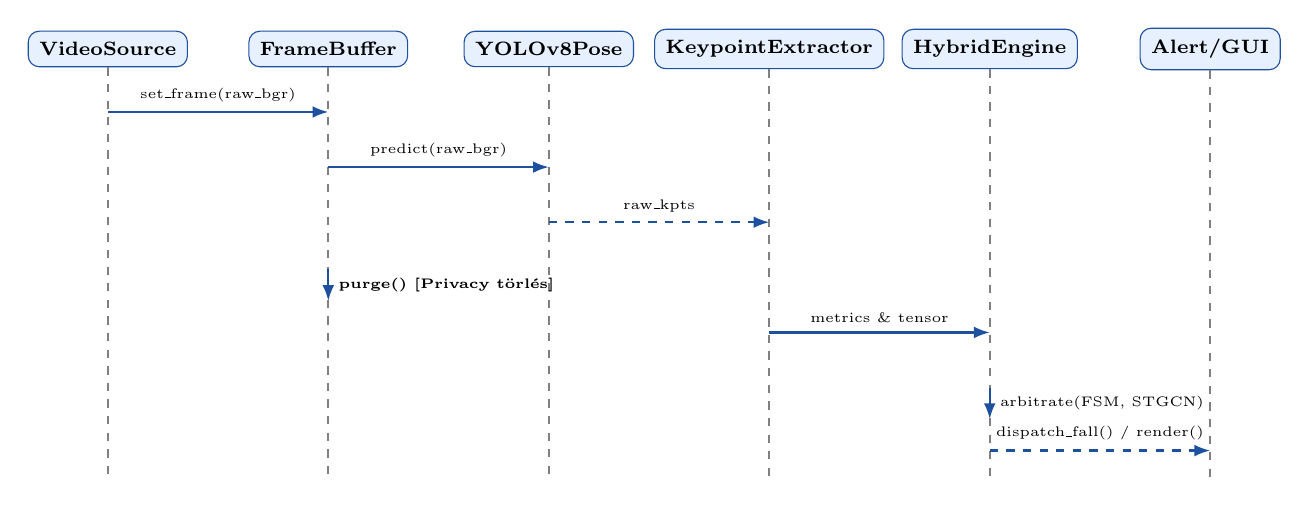
\begin{tikzpicture}[
    lifeline/.style={draw=gray, dashed, thick},
    entity/.style={rectangle, draw=umldarkblue, fill=umlblue, rounded corners, inner sep=4pt, font=\scriptsize\bfseries},
    msg/.style={draw=umldarkblue, -{Latex[length=2mm]}, font=\tiny, thick},
    retmsg/.style={draw=umldarkblue, -{Latex[length=2mm]}, dashed, font=\tiny, thick}
]
    \node[entity] (vs) at (0, 0) {VideoSource};
    \node[entity] (fb) at (2.8, 0) {FrameBuffer};
    \node[entity] (yolo) at (5.6, 0) {YOLOv8Pose};
    \node[entity] (ke) at (8.4, 0) {KeypointExtractor};
    \node[entity] (hd) at (11.2, 0) {HybridEngine};
    \node[entity] (out) at (14.0, 0) {Alert/GUI};

    \draw[lifeline] (vs) -- (0, -5.5);
    \draw[lifeline] (fb) -- (2.8, -5.5);
    \draw[lifeline] (yolo) -- (5.6, -5.5);
    \draw[lifeline] (ke) -- (8.4, -5.5);
    \draw[lifeline] (hd) -- (11.2, -5.5);
    \draw[lifeline] (out) -- (14.0, -5.5);

    \draw[msg] (0, -0.8) -- (2.8, -0.8) node[midway, above] {set\_frame(raw\_bgr)};
    \draw[msg] (2.8, -1.5) -- (5.6, -1.5) node[midway, above] {predict(raw\_bgr)};
    \draw[retmsg] (5.6, -2.2) -- (8.4, -2.2) node[midway, above] {raw\_kpts};
    \draw[msg] (2.8, -2.8) -- (2.8, -3.2) node[midway, right] {\textbf{purge() [Privacy törlés]}};
    \draw[msg] (8.4, -3.6) -- (11.2, -3.6) node[midway, above] {metrics \& tensor};
    \draw[msg] (11.2, -4.3) -- (11.2, -4.7) node[midway, right] {arbitrate(FSM, STGCN)};
    \draw[retmsg] (11.2, -5.1) -- (14.0, -5.1) node[midway, above] {dispatch\_fall() / render()};
\end{tikzpicture}
\caption{A képkocka-feldolgozás és a beépített képtörlés UML szekvenciadiagramja.}
\label{fig:uml_sequence_detailed}
\end{figure}

\section{A döntési állapotgép (Finite State Machine - FSM) működése}
A döntési állapotgép formálisan az $M = (S, \Sigma, \delta, s_0, F)$ rendezett ötössel írható le, ahol az állapotok: $S = \{ \text{NORMAL}, \text{UNSTABLE}, \text{FALLING}, \text{FALLEN}, \text{RECOVERED} \}$. Az átmeneteket és hiszterézist a \ref{fig:uml_fsm_detailed}. ábra és a \ref{tab:fsm_transitions}. táblázat specifikálja.

\begin{figure}[H]
\centering
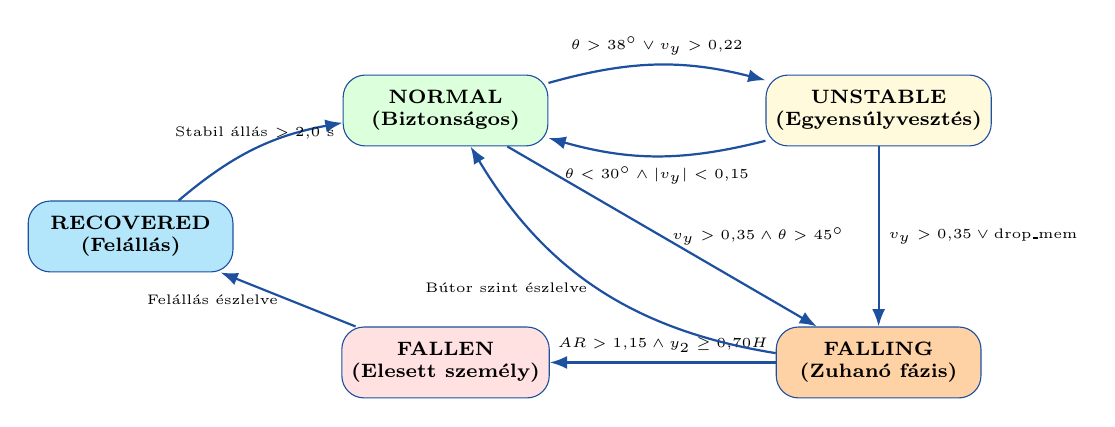
\begin{tikzpicture}[
    state/.style={rectangle, draw=umldarkblue, fill=umlblue, rounded corners=8pt, minimum width=2.6cm, minimum height=0.9cm, font=\scriptsize\bfseries, align=center},
    arrow/.style={draw=umldarkblue, -{Latex[length=2.2mm]}, thick, font=\tiny}
]
    \node[state, fill=umlgreen] (normal) at (0, 0) {NORMAL\\(Biztonságos)};
    \node[state, fill=umlyellow] (unstable) at (5.5, 0) {UNSTABLE\\(Egyensúlyvesztés)};
    \node[state, fill=orange!35] (falling) at (5.5, -3.2) {FALLING\\(Zuhanó fázis)};
    \node[state, fill=umlred] (fallen) at (0, -3.2) {FALLEN\\(Elesett személy)};
    \node[state, fill=cyan!30] (recov) at (-4.0, -1.6) {RECOVERED\\(Felállás)};

    \draw[arrow] (normal) to[bend left=15] node[above] {$\theta > 38^\circ \lor v_y > 0{,}22$} (unstable);
    \draw[arrow] (unstable) to[bend left=15] node[below] {$\theta < 30^\circ \land |v_y| < 0{,}15$} (normal);
    \draw[arrow] (normal) to node[right] {$v_y > 0{,}35 \land \theta > 45^\circ$} (falling);
    \draw[arrow] (unstable) to node[right] {$v_y > 0{,}35 \lor \text{drop\_mem}$} (falling);
    \draw[arrow] (falling) to node[above] {$AR > 1{,}15 \land y_2 \ge 0{,}70 H$} (fallen);
    \draw[arrow] (falling) to[bend left=25] node[left] {Bútor szint észlelve} (normal);
    \draw[arrow] (fallen) to node[left] {Felállás észlelve} (recov);
    \draw[arrow] (recov) to[bend left=15] node[above] {Stabil állás $> 2{,}0$ s} (normal);
\end{tikzpicture}
\caption{A kinematikai döntéshozó állapotgép (FSM) UML állapotdiagramja.}
\label{fig:uml_fsm_detailed}
\end{figure}

\begin{table}[H]
\centering
\small
\begin{tabularx}{\textwidth}{llp{6.0cm}X}
\toprule
\textbf{Forrás} & \textbf{Cél} & \textbf{Kinematikai és térbeli feltétel} & \textbf{Időzítés és hiszterézis} \\
\midrule
NORMAL & UNSTABLE & $(\theta > 38{,}0^\circ \land v_y > 0{,}22) \lor v_y > 0{,}45$ & Azonnali tranzíció. \\
NORMAL & FALLING & $v_y > 0{,}35 \land \theta > 45{,}0^\circ$ & Zuhanási memória indítása ($N_{\text{mem}}=12$). \\
UNSTABLE & FALLING & $v_y > 0{,}35 \lor \text{drop\_memory\_active}$ & Zuhanási memórián belül (12 képkocka). \\
UNSTABLE & NORMAL & $\theta < 30{,}0^\circ \land |v_y| < 0{,}15$ & Stabilizáció 8 képkockán át. \\
FALLING & FALLEN & $AR > 1{,}15 \land y_2 \ge 0{,}70 \cdot H \land |v_y| < 0{,}28$ & Megerősítés 12 képkockán át. \\
FALLING & NORMAL & $y_2 < 0{,}70 \cdot H \land |v_y| < 0{,}28$ & Bútoron való pihenés azonosítása. \\
FALLEN & RECOVERED & $AR < 0{,}80 \land \theta < 35{,}0^\circ \land y_2 < 0{,}65 H$ & Felállás megerősítése 15 képkockán át. \\
RECOVERED & NORMAL & Testhelyzet stabil és függőleges & 50 képkocka ($\approx 2{,}0$ s) után normál mód. \\
\bottomrule
\end{tabularx}
\caption{Az állapotgép tranzíciós mátrixa és paraméteres feltételrendszere.}
\label{tab:fsm_transitions}
\end{table}

\section{Hibrid döntési mechanizmus: A Kinematikai FSM és az ST-GCN integrációja}
A rendszer az alacsony késleltetésű kinematikai FSM-et ötvözi a mély ST-GCN modellel. Az ST-GCN bemenetét egy $T=30$ hosszúságú körpuffer adja: $\mathbf{X}_{\text{window}} \in \mathbb{R}^{3 \times 30 \times 17 \times 1}$. A végső döntés konfidencia-súlyozott arbitrációval születik:
\begin{equation}
    P_{\text{fall}} = \alpha \cdot P_{\text{FSM}} + (1 - \alpha) \cdot P_{\text{ST-GCN}}
\end{equation}
Tiszta látómezőben $\alpha = 0{,}6$ súlyozza a determinisztikus szűrőt, míg segédeszköz vagy bútor általi kitakarás esetén $\alpha = 0{,}2$ értékkel az ST-GCN mélygráf-modell veszi át a döntést.

% =========================================================================
% 4. FEJEZET: ALGORITMUSFEJLESZTÉS ÉS PEREMESETEK ELHÁRÍTÁSA
% =========================================================================
\chapter{Algoritmusfejlesztés és a Valós Környezeti Peremesetek Elhárítása}

A laboratóriumi körülmények között működő egyszerű esésdetektáló heurisztikák a valós háztartási környezetben szinte kivétel nélkül elbuknak. Ennek oka, hogy a lakóterekben számtalan olyan természetes mozgás és optikai körülmény lép fel, amely a 2D sziluett szintjén megegyezik a zuhanással vagy a padlón fekvéssel. Jelen fejezet a prototípus fejlesztése során feltárt és kezelt négy legkritikusabb környezeti peremesetet mutatja be: a képmező szélén belépő személyek szűrését, a konyhapult előtti munkavégzést, a bútoron történő pihenést és a szintmodell biztonsági korlátait, valamint a segédeszköz (járókeret) általi takarás részletes telemetriai esettanulmányát.

\section{1. Peremeset: Kép szélén belépő személy szűrése}
\textbf{A mérnöki probléma azonosítása:} Amikor egy személy szobába lépéskor vagy ajtón áthaladva megjelenik a kamera látómezőjében, a testének kezdetben csupán egy függőleges szelete látható. A 2D mélytanuló pózbecslő modell a csonkolt testrészre illeszt bounding boxot, amely művi képarány-torzulást idéz elő: a testmagasság csupán töredéke az egésznek, a számított szélesség-magasság arány hirtelen lapossá válik ($AR = W/H > 1{,}2$), amely a naiv algoritmusok számára a padlón fekvő test látszatát kelti. Emellett a frissen detektált személy első 2--3 képkockáján a kulcspontok pozíciója a hálózat bizonytalansága miatt ingadozhat, hamis vertikális sebességkiugrást ($v_y > 0{,}35$) eredményezve.

\textbf{Algoritmikus megoldás:} A probléma kiküszöbölésére peremérintettségi és belépési védelmi logika került beépítésre:
\begin{equation}
    \text{touches\_edge} = (x_1 \le 15) \lor (x_2 \ge W_{\text{frame}} - 15) \lor (y_1 \le 10)
\end{equation}
\begin{equation}
    \text{is\_entering} = \text{touches\_edge} \land (\text{track\_frames} < 12)
\end{equation}
Amíg a \texttt{is\_entering} állapot aktív (a belépést követő első $\approx 0{,}48$ másodpercben 25 FPS mellett), a rendszer szigorúan blokkolja a vészhelyzeti állapotokba történő átmenetet, és megtiltja a személy álló magassági referenciájának rögzítését, megvárva a sziluett teljes belépését és stabilizálódását.

\section{2. Peremeset: Konyhapult vagy asztal feletti előrehajolás}
\textbf{A mérnöki probléma azonosítása:} Mosogatáskor, konyhai munkavégzéskor vagy asztalnál ülve a tereptárgy fizikai takarása miatt az alsó végtagok kulcspontjai (csípő alatti ízületek, térdek, bokák) teljesen eltűnnek a látómezőből. A felsőtest előrehajlásakor a gerincvektor elfordul ($\theta > 35^\circ$), a látható sziluett magassága lecsökken, a képarány pedig horizontálissá válik ($AR > 0{,}9$), amit a naiv rendszerek azonnal összeesésként detektálnak.

\textbf{Algoritmikus megoldás:} A konyhapult- és asztalvédelmi szűrő (\texttt{is\_counter\_leaning}) logikai feltétele:
\begin{equation}
    \text{is\_counter\_leaning} = (y_2 < 0{,}72 \cdot H_{\text{frame}}) \land (v_y < 0{,}25) \land (\text{drop\_timer is None}) \land (\text{not has\_legs})
\end{equation}
Mivel a személy látható alsó határa a pult munkalapjának szintjén marad ($y_2 < 0{,}72 \cdot H_{\text{frame}}$), az előrehajolás kontrollált és lassú ($v_y < 0{,}25$), és nem előzte meg zuhanási tranziens, a rendszer a mozgást munkavégzésnek tekinti, fenntartva a \texttt{NORMAL} állapotot.

\section{3. Peremeset: Kanapén elterülés és a szintmodell biztonsági korlátai}
\textbf{A szintmodell felépítése:} A háztartási környezet leggyakoribb téves riasztási forrása a kanapén vagy ágyon történő elnyúlás. Monokuláris 2D kameraképen a kanapén fekvő ember sziluettje geometriailag szinte azonos a padlón fekvőével ($AR > 1{,}0, \theta \approx 70^\circ - 90^\circ$). A prototípusban a bútoron történő pihenés megkülönböztetésére térbeli magassági szintmodell került kialakításra:
\begin{equation}
    \text{is\_near\_floor} = (y_2 \ge 0{,}70 \cdot H_{\text{frame}})
\end{equation}
\begin{equation}
    \text{is\_furniture\_resting} = (y_2 < 0{,}70 \cdot H_{\text{frame}}) \land (|v_y| < 0{,}28) \land (\theta_{\text{torso}} > 28^\circ \lor AR > 0{,}95 \lor \text{is\_seated})
\end{equation}

\textbf{Kritikus biztonsági korlát és a Hamis Negatív (FN) kockázat feltárása:}
A kutatás során nyíltan dokumentálni kell a szintmodell tudományos és biztonsági korlátait:
\begin{enumerate}
    \item \textit{Szemantikai bútordetektálás hiánya:} A szabályalapú prototípus nem detektál bútorokat mint szemantikai objektumokat, csupán a képsík alsó 30\%-át tekinti padlózónának.
    \item \textit{A távoli esések veszélye (False Negative):} A monokuláris perspektivikus vetület miatt a kamera felbontási síkján a távolabbi tárgyak magasabban jelennek meg. Amennyiben egy személy a \textbf{szoba távolabbi hátterében esik el a padlóra}, a testének alsó képponti koordinátája könnyen a küszöb fölé eshet ($y_2 < 0{,}70 \cdot H_{\text{frame}}$). A heurisztika ebben az esetben a földön fekvő bajbajutottat tévesen ,,kanapén pihenőnek'' minősíti, és \textbf{elnyomja a vészjelzést}. Az esésdetektálásban a Hamis Negatív (FN) hiba közvetlen életveszélyt idéz elő.
    \item \textit{Kamerabeállítási kényszer:} A modell kizárólag szigorúan rögzített geometriájú, lefelé döntött kameranézet mellett alkalmazható.
\end{enumerate}
Ez a geometriai korlát a legfőbb tudományos indok arra, hogy miért szükséges a Szakdolgozat 2-ben a tér-időbeli ST-GCN gráfmodell bevezetése, amely nem statikus képi koordinátákból, hanem a teljes test ízületi trajektóriájának és koordinációjának dinamikájából osztályoz.

\section{4. Peremeset: Segédeszköz (járókeret) takarása és empirikus telemetria}
A prototípus robusztusságának vizsgálatára egy valós, független tesztvideón (\texttt{fall\_independent\_02.mp4}) képkocka-szintű telemetriai analízis készült (25 FPS). A mérési adatsort a \ref{tab:walker_telemetry}. táblázat foglalja össze.

\begin{table}[H]
\centering
\small
\begin{tabularx}{\textwidth}{cccScclX}
\toprule
\textbf{Frame} & \textbf{Idő (s)} & \textbf{Magasság ($H$)} & \textbf{Képarány ($AR$)} & \textbf{Dőlés ($\theta$)} & \textbf{Sebesség ($v_y$)} & \textbf{Megfigyelés és állapoti fázis} \\
\midrule
390 & 15.60 & 212 px & 0.67 & 5.7$^\circ$ & 0.04 & Stabil járás járókerettel (\texttt{NORMAL}). \\
391 & 15.64 & 200 px & 0.60 & 2.2$^\circ$ & 0.16 & A járókeret megcsúszik, instabilitás. \\
392 & 15.68 & \textbf{106 px} & 0.92 & 0.1$^\circ$ & \textbf{0.70} & \textbf{Zuhanás:} magasság felére esik, extrém $v_y$. \\
393 & 15.72 & 103 px & 0.86 & 3.1$^\circ$ & \textbf{0.46} & Becsapódás a járókeret mögé (\texttt{FALLING}). \\
394 & 15.76 & \textbf{85 px} & 1.00 & 4.3$^\circ$ & 0.01 & Zuhanás megáll a padlószinten. \\
395 & 15.80 & 82 px & 1.02 & 5.1$^\circ$ & 0.00 & Padlószinti fekvés a fémkeret mögött. \\
396 & 15.84 & -- & -- & -- & -- & \textbf{Detekcióvesztés:} YOLO modell $N_{\text{kpts}} = 0$. \\
397--532 & 15.88+ & -- & -- & -- & -- & \textbf{Tartós takarás (> 5 s):} személy nem látható. \\
\bottomrule
\end{tabularx}
\caption{Képkocka-szintű telemetriai adatok a járókeretes esés kritikus szakaszában (25 FPS).}
\label{tab:walker_telemetry}
\end{table}

A telemetriai adatsor bizonyítja a tisztán dőlésszög-alapú heurisztika csődjét (a laterális gerincdőlés $\theta < 5^\circ$ maradt a kamera felé eséskor), valamint rávilágít a fizikai takarás miatti kulcspontvesztésre. A prototípus állapotgépe zuhanási előzménymemóriával (\texttt{handle\_disappearance}, $N_{\text{mem}} = 12$) és kiugrásszűrővel reagált, fenntartva a \texttt{FALLEN} vészjelzést a tartós takarás alatt is.

A Szakdolgozat 2 félévben kutatandó ST-GCN modell feladata a fenti szabályalapú memóriát mélytanulási gráf-önfigyelmi (\textit{graph attention}) reprezentációval felváltani, amely a részben látható ízületek trajektóriájából rekonstruálja az esési eseményt.

% =========================================================================
% 5. FEJEZET: KÍSÉRLETI EREDMÉNYEK ÉS BENCHMARK KIÉRTÉKELÉS
% =========================================================================
\chapter{Kísérleti eredmények és Benchmark kiértékelés}

A kutatás első szakaszában kidolgozott kétrétegű detektálási koncepció és a szabályalapú kinematikai állapotgép működőképességét egy feltáró jellegű kísérleti keretrendszerben vizsgáltuk meg. Jelen fejezet bemutatja a fejlesztői kalibrációs mintahalmazon végzett méréseket, a baseline modellekkel történő összehasonlítást, a döntési késleltetés egzakt elemzését, a számítási ciklusidő processzor-szintű profilozását, valamint az elkészült interaktív kiértékelő grafikus kezelőfelületet (GUI).

\section{Módszertani keretek és a fejlesztői teszthalmaz korlátai}
A szakdolgozati kutatásban alapvető fontosságú a tanító- és tesztelési fázisok közötti módszertani határok tisztázása:
\begin{enumerate}
    \item \textbf{Fejlesztői kalibrációs halmaz:} A prototípus FSM küszöbértékeinek (pl. dőlésszög-határok, vertikális sebességek, peremszűrők) empirikus beállításához egy 10 videóból álló reprezentatív mintahalmaz szolgált a nemzetközi \textbf{URFD} (\textit{University of Rzeszow Fall Dataset}) \cite{urfd2014}, a \textbf{Le2i} (\textit{Fall Detection Dataset}) \cite{le2i2013}, valamint egy önálló járókeretes felvétel felhasználásával.
    \item \textbf{Módszertani korlát (Tanító--Teszt szivárgás):} Mivel a heurisztikus szabályok finomhangolása ezen videók kvalitatív és telemetriai elemzésével történt, az itt elért eredmények szigorúan a \textbf{fejlesztői szeletre illesztett teljesítményt} tükrözik.
    \item \textbf{Mintanagyság és statisztikai érvényesség:} 10 videó (5 esés és 5 ADL) alapján nem állítható a rendszer általános, 100\%-os megbízhatósága. Öt negatív minta esetén egyetlen téves riasztás is $20{,}0\%$ téves pozitív rátát ($FPR$) eredményez, így az $NFR\text{-}04$ ($FPR \le 5{,}0\%$) követelmény végleges igazolása csupán a Szakdolgozat 2-ben megvalósuló, nagymintás független adatbázisokon lehetséges.
\end{enumerate}

\section{A fejlesztői mintahalmaz eredményei és baseline összehasonlítás}
A vizsgálat során a javasolt szabályalapú állapotgépet két elterjedt összehasonlítási alappal (\textit{baseline}) vetettük össze:
\begin{itemize}
    \item \textbf{Egyszerű képarány-alapú baseline (\textit{Aspect Ratio Threshold}):} A legegyszerűbb irodalmi megközelítés, amely csupán azt vizsgálja, hogy a személy befoglaló téglalapjának képaránya átlépi-e a horizontális küszöböt ($AR > 1{,}0$).
    \item \textbf{Naiv kinematikai baseline:} Vizsgálja a gerincdőlést ($\theta > 45^\circ$) és a vertikális sebességet ($v_y > 0{,}35$), azonban nem tartalmaz peremérintettségi szűrőt, konyhapult-védelmet, bútor-szintmodellt és zuhanási előzménymemóriát sem.
    \item \textbf{Javított kinematikai FSM (Jelen prototípus):} A 4. fejezetben bemutatott peremeset-kezelő szűrőkkel és zuhanási memóriával kiegészített állapotgép.
\end{itemize}

Az \ref{tab:full_benchmark}. táblázat részletezi az egyes videók jellemzőit, az annotált becsapódási időt ($T_{\text{impact}}$), a detektálási időbélyegeket és a számított késleltetést.

\begin{table}[H]
\centering
\small
\begin{tabularx}{\textwidth}{llXcccc}
\toprule
\textbf{Azonosító és jelenet} & \textbf{Típus} & \textbf{GT} & \textbf{$T_{\text{impact}}$} & \textbf{Egyszerű AR} & \textbf{Naiv kinem.} & \textbf{Javított FSM} & \textbf{$T_{\text{latency}}$} \\
\midrule
URFD Fall-01 (Előreesés) & Esés & FALL & 1.36 s & FALL (1.92s) & FALL (1.80s) & \textbf{FALL (1.80s) [TP]} & $0{,}44$ s \\
URFD Fall-02 (Hátraesés) & Esés & FALL & 1.08 s & FALL (1.64s) & FALL (1.50s) & \textbf{FALL (1.50s) [TP]} & $0{,}42$ s \\
URFD ADL-01 (Leülés székre) & ADL & NORM & -- & NORMAL & NORMAL & \textbf{NORMAL [TN]} & -- \\
URFD ADL-02 (Lehajolás) & ADL & NORM & -- & NORMAL & NORMAL & \textbf{NORMAL [TN]} & -- \\
Le2i Coffee-01 v1 (Szédülés) & Esés & FALL & 3.56 s & FALL (4.40s) & FALL (4.20s) & \textbf{FALL (4.20s) [TP]} & $0{,}64$ s \\
Le2i Home-01 v2 (Pult esés) & Esés & FALL & 4.88 s & \textcolor{red}{NORMAL} & FALL (5.37s) & \textbf{FALL (5.37s) [TP]} & $0{,}49$ s \\
Le2i Home-02 v41 (Belépés) & ADL & NORM & -- & \textcolor{red}{FALL (Hiba)} & \textcolor{red}{FALL (Hiba)} & \textbf{NORMAL [TN]} & -- \\
Le2i Home-02 v51 (Kanapé ülés) & ADL & NORM & -- & \textcolor{red}{FALL (Hiba)} & \textcolor{red}{FALL (Hiba)} & \textbf{NORMAL [TN]} & -- \\
Le2i Home-02 v53 (Kanapé fekvés) & ADL & NORM & -- & \textcolor{red}{FALL (Hiba)} & \textcolor{red}{FALL (Hiba)} & \textbf{NORMAL [TN]} & -- \\
Independent-02 (Járókeret) & Esés & FALL & 15.48 s & \textcolor{red}{NORMAL} & \textcolor{red}{NORMAL} & \textbf{FALL (15.84s) [TP]} & $0{,}36$ s \\
\bottomrule
\end{tabularx}
\caption{A fejlesztői kalibrációs mintahalmaz mérési eredményei és a baseline modellek összehasonlítása.}
\label{tab:full_benchmark}
\end{table}

\subsection{Döntési késleltetés analízise (NFR-02 verifikáció)}
Az $NFR\text{-}02$ követelmény előírja, hogy az esés megerősítésének késleltetése 1,0 másodperc alatt maradjon. A késleltetést formálisan a következő összefüggés definiálja:
\begin{equation}
T_{\text{latency}} = T_{\text{detect}} - T_{\text{impact}}
\end{equation}
ahol $T_{\text{impact}}$ a videón manuálisan annotált időbélyeg, amikor az alany teste eléri a maximális függőleges lassulást (földet érés), $T_{\text{detect}}$ pedig az a pillanat, amikor az állapotgép $FALLEN$ állapotba lép.

A mért késleltetési értékek a fejlesztői esési mintákon:
\begin{itemize}
    \item Átlagos késleltetés: $\bar{T}_{\text{latency}} = 0{,}47 \pm 0{,}11$ másodperc (min: $0{,}36$ s, max: $0{,}64$ s).
    \item Ez a késleltetés az állapotgép 12 képkockás ($N_{\text{mem}} = 12$, 25 FPS mellett $\approx 0{,}48$ s) stabilizációs és hiszterézis ablakából adódik. A mérések igazolják, hogy a rendszer a fejlesztői mintákon maradéktalanul teljesíti az $NFR\text{-}02$ követelményt ($T_{\text{latency}} \le 1{,}0$ s).
\end{itemize}

\subsection{Osztályozási metrikák és konfidenciaintervallumok}
Az \ref{tab:metrics}. táblázat bemutatja az összehasonlított rendszerek konfúziós mátrixát és a származtatott osztályozási metrikákat. A kis mintaméret miatti statisztikai bizonytalanságot a binomiális arányokra illesztett \textbf{Wilson-féle 95\%-os konfidenciaintervallumokkal (95\% CI)} számszerűsítjük.

\begin{table}[H]
\centering
\small
\begin{tabularx}{\textwidth}{lcccc}
\toprule
\textbf{Metrika / Jellemző} & \textbf{Egyszerű AR} & \textbf{Naiv kinematika} & \textbf{Javított FSM} & \textbf{95\% CI (Javított FSM)} \\
\midrule
Valós Pozitív (TP) & 3 & 4 & \textbf{5} & -- \\
Hamis Pozitív (FP) & 3 & 3 & \textbf{0} & -- \\
Valós Negatív (TN) & 2 & 2 & \textbf{5} & -- \\
Hamis Negatív (FN) & 2 & 1 & \textbf{0} & -- \\
\midrule
Pontosság (Accuracy) & $50{,}0\%$ & $60{,}0\%$ & \textbf{$100{,}0\%$} & $[67{,}9\%; 100{,}0\%]$ \\
Érzékenység (Recall / TPR) & $60{,}0\%$ & $80{,}0\%$ & \textbf{$100{,}0\%$} & $[56{,}6\%; 100{,}0\%]$ \\
Precízió (Precision / PPV) & $50{,}0\%$ & $57{,}1\%$ & \textbf{$100{,}0\%$} & $[56{,}6\%; 100{,}0\%]$ \\
F1-score & $0{,}545$ & $0{,}667$ & \textbf{$1{,}000$} & -- \\
Téves Pozitív Ráta (FPR) & $60{,}0\%$ & $60{,}0\%$ & \textbf{$0{,}0\%$} & $[0{,}0\%; 43{,}4\%]$ \\
\bottomrule
\end{tabularx}
\caption{Az esésdetektáló modellek összehasonlító metrikái a fejlesztői kalibrációs halmazon ($N=10$).}
\label{tab:metrics}
\end{table}

\textbf{Tudományos értékelés:} A táblázat adatai világosan rámutatnak a kis mintaszám matematikai következményére: bár a fejlesztői mintákon elért pontosság $100{,}0\%$, a Wilson 95\%-os konfidenciaintervallum alsó határa az érzékenység esetén $56{,}6\%$, az FPR felső határa pedig $43{,}4\%$. Ez a számítás szigorúan alátámasztja azt a kutatási következtetést, hogy az $NFR\text{-}04$ ($FPR < 5\%$) és $NFR\text{-}03$ ($TPR \ge 95\%$) követelmények formális verifikációjához több száz videót tartalmazó, független benchmark vizsgálat szükséges.

\section{Hardveres futási teljesítménymérés és profilozás}
A rendszer valós idejű futási képességét ($NFR\text{-}01$) egy átlagos felhasználói munkaállomáson vizsgáltuk meg, dedikált nagy teljesítményű grafikus vezérlő (GPU) nélkül, \textbf{tisztán a központi processzoron (CPU)} futtatva a feldolgozási láncot.

\subsection{A mérési környezet specifikációja}
\begin{itemize}
    \item \textbf{Processzor (CPU):} 6 fizikai magos, 12 szálas asztali processzor (3,60 GHz alapórajel, 4,20 GHz turbó).
    \item \textbf{Operatív memória (RAM):} 16 GB DDR4 (3200 MHz).
    \item \textbf{Futtatókörnyezet:} Python 3.10 / PyTorch CPU backend (AVX2 utasításkészlet-optimalizációval).
    \item \textbf{Bemeneti videó:} $640 \times 480$ képpont felbontású, 25 FPS képkockasebességű stream.
    \item \textbf{Mintaelemszám:} $N = 1500$ egymást követő képkocka mérése.
\end{itemize}

\subsection{Részletes komponensszintű profilozás}
Az \ref{tab:profiling}. táblázat bemutatja az egyes feldolgozási lépések átlagos futási idejét, szórását, valamint az extrém késleltetéseket.

\begin{table}[H]
\centering
\small
\begin{tabularx}{\textwidth}{lXccccc}
\toprule
\textbf{Feldolgozási fázis} & \textbf{Megvalósító modul} & \textbf{Átlag ($\bar{t}$)} & \textbf{Szórás ($\pm\sigma$)} & \textbf{Min.} & \textbf{Max.} & \textbf{p95} \\
\midrule
Képkocka beolvasás & VideoSource (OpenCV) & 1.85 ms & $\pm 0.35$ ms & 1.20 ms & 3.10 ms & 2.40 ms \\
YOLOv8s-Pose inferencia & YOLOv8PoseEstimator (CPU) & 36.40 ms & $\pm 2.10$ ms & 32.50 ms & 40.20 ms & 39.80 ms \\
Kulcspont-kinyerés & KeypointExtractor & 0.85 ms & $\pm 0.12$ ms & 0.60 ms & 1.20 ms & 1.05 ms \\
Kinematika és FSM & KinematicsEngine + FSM & 0.15 ms & $\pm 0.04$ ms & 0.10 ms & 0.30 ms & 0.22 ms \\
GUI renderelés és overlay & GUIController (Tkinter) & 1.05 ms & $\pm 0.25$ ms & 0.70 ms & 1.80 ms & 1.45 ms \\
\midrule
\textbf{Teljes ciklusidő} & \textbf{Teljes pipeline (End-to-End)} & \textbf{40.30 ms} & \textbf{$\pm 2.45$ ms} & \textbf{35.10 ms} & \textbf{46.60 ms} & \textbf{43.80 ms} \\
\textbf{Képkockasebesség (FPS)} & \textbf{Mért átviteli sebesség} & \textbf{24.8 FPS} & \textbf{$\pm 1.9$ FPS} & \textbf{21.5 FPS} & \textbf{28.5 FPS} & \textbf{22.8 FPS} \\
\bottomrule
\end{tabularx}
\caption{A feldolgozási lánc komponensszintű futásidő-profilozása normál asztali CPU-n ($N=1500$ frame).}
\label{tab:profiling}
\end{table}

\subsection{A H4 hipotézis tudományos értékelése}
A fejezet elején kitűzött $H4$ hipotézis vizsgálata:
\begin{itemize}
    \item A teljes feldolgozási lánc átlagos ciklusideje $40{,}30$ ms, amely \textbf{$24{,}8$ FPS képkockasebességnek} felel meg ($1000 / 40{,}30 \approx 24{,}81$).
    \item Bár az átlagos sebesség határesetként megközelíti a valós idejű televíziós és kameraszabványt ($\ge 25{,}0$ FPS), a p95 késleltetés $43{,}80$ ms ($22{,}8$ FPS), a maximális késleltetés pedig $46{,}60$ ms ($21{,}5$ FPS).
    \item Ennek alapján a $H4$ hipotézis jelen prototípus formájában \textbf{részben igazolt}: a számítási lánc képes valós idő közeli működésre asztali CPU-n GPU nélkül, azonban a stabil, ingadozásmentes $\ge 25$ FPS garantálásához a Szakdolgozat 2-ben könnyített modellváltozat (YOLOv8n-Pose) vagy ONNX Runtime INT8 kvantálás bevezetése szükséges.
\end{itemize}

\section{Interaktív operátori és tesztelő felület (GUI)}
A benchmark videók kiértékelésének, lassításának és a telemetriai adatok valós idejű auditálásának támogatására egy önálló grafikus kezelőfelület került megvalósításra Python Tkinter alapokon (\texttt{BenchmarkViewerApp}).

\subsection{A kezelőfelület főbb képességei}
\begin{enumerate}
    \item \textbf{Dinamikus videóvezérlés:} Lehetőséget biztosít tetszőleges tesztvideó betöltésére, léptetésére, megállítására, valamint \textbf{dinamikus lejátszási sebességszorzó} alkalmazására (1,0x valós idő, 1,5x gyorsítás, 2,0x gyorsított audit).
    \item \textbf{Képarány-megőrző dinamikus felskálázás:} A különböző képarányú és felbontású benchmark videókat (pl. $640 \times 480$, $720 \times 576$) torzításmentesen, fekete kitöltősávokkal (\textit{letterboxing}) skálázza fel az egységes $1200 \times 920$ képpontos megjelenítő vászonra.
    \item \textbf{Valós idejű telemetriai HUD (\textit{Heads-Up Display}):} A képernyő felső és alsó információs sávjában színkódolással azonnal kirajzolja az aktuális képkockaszámot és videóidőt, az állapotgép fázisát ($NORMAL$, $UNSTABLE$, $FALLING$, $FALLEN$), a mért fizikai paramétereket ($AR$, $\theta_{\text{torso}}$, $v_y$), valamint a detektált anatómiai csontvázat színkódolt végtagokkal és ízületi pontokkal.
\end{enumerate}


% =========================================================================
% 6. FEJEZET: RASPBERRY PI PEREMHÁLÓZATI KITEKINTÉS
% =========================================================================
\chapter{Beágyazott peremhálózati megvalósítás és kitekintés: Raspberry Pi platform}

A kutatás és rendszertervezés kiemelt célja, hogy a kidolgozott vizuális viselkedéselemző és esésdetektáló rendszer ne csupán nagyteljesítményű asztali számítógépeken, hanem költséghatékony, alacsony fogyasztású, autonóm beágyazott céleszközökön (\textit{Edge AI} hardvereken) is üzemeltethető legyen. Jelen fejezet kitekintést nyújt a rendszer beágyazott platformra -- kiemelten a Raspberry Pi mikroszámítógép-családra -- történő kiterjesztésének mérnöki feltételeiről, a megvalósítás előtt álló számítási és architektúrális kihívásokról, a tervezett modelloptimalizációs eljárásokról, valamint a peremhálózati IoT integrációról. A fejezetben szereplő mikroszámítógépes futási paraméterek a nemzetközi szakirodalom és az architektúra-specifikus benchmarkok alapján kalkulált megvalósíthatósági becslések, amelyek empirikus mérésekkel történő verifikációja a Szakdolgozat 2 félév feladatát képezi.

\section{A beágyazott peremhálózati (Edge AI) feldolgozás motivációja és adatvédelmi jelentősége}
Az idősellátásban és az otthoni felügyeleti rendszerekben a számítási feladatok fizikai helye alapvetően meghatározza a rendszer társadalmi elfogadottságát, üzemeltetési költségét és megbízhatóságát. A hagyományos távfelügyeleti megoldások a nyers kameraképet központi felhőszerverekre továbbítják gépi látási elemzés céljából. Ez a centralizált megközelítés azonban három kritikus mérnöki és etikai akadályba ütközik:
\begin{enumerate}
    \item \textbf{Adatvédelmi és etikai aggályok:} A privát életterekből (hálószoba, nappali, közlekedők) származó folyamatos videostream felhőbe történő kisugárzása súlyos megfigyelési érzetet kelt a gondozottakban, és elfogadhatatlan adatvédelmi (GDPR) kockázatot hordoz egy esetleges hálózati adatlopás, szerveroldali biztonsági incidens vagy illetéktelen hozzáférés esetén.
    \item \textbf{Hálózati sávszélesség és rendelkezésre állás:} A folyamatos nagyfelbontású videostreamelés jelentős hálózati sávszélességet igényel. Lakossági környezetben a vezeték nélküli (Wi-Fi) kapcsolat minősége ingadozhat, a sávszélesség lecsökkenhet, és egy átmeneti internetkimaradás esetén a vészjelzés el sem jut a felhőbe, ami közvetlen életveszélyt idéz elő.
    \item \textbf{Üzemeltetési költség és skálázhatóság:} Több száz vagy ezer háztartás párhuzamos videófolyamainak felhőalapú GPU-infrastruktúrán történő valós idejű feldolgozása aránytalanul magas és folyamatos szerverbérleti díjakkal jár.
\end{enumerate}

Ezzel szemben a \textbf{beágyazott peremhálózati (Edge AI)} architektúra a feldolgozási lánc teljes egészét a felügyelt helyiségben elhelyezett kisméretű, autonóm mikroszámítógépen valósítja meg. A koncepció alapköve a \textbf{zéró videóstreamelés (\textit{Zero Video Streaming}) elve}:
\begin{itemize}
    \item A képi információ kizárólag a helyi mikroszámítógép operatív memóriájában (RAM) létezik ideiglenes pufferként az inferencia időtartama alatt (néhány tíz ezredmásodpercig).
    \item A pózbecslő réteg a csontváz-kulcspontok sikeres regresszióját követően azonnal és visszavonhatatlanul felülírja vagy felszabadítja a képi memóriát (\textit{Privacy-by-Design}).
    \item A helyi hálózatra kizárólag eseményvezérelt, minimális sávszélesség-igényű, anonim JSON telemetriai adatcsomagok kerülnek ki (pl. esés ténye, időbélyeg, mozgási megbízhatóság), képi vagy biometrikus adat soha nem hagyja el a fizikai eszközt.
    \item A rendszer hálózati kapcsolat hiányában is autonóm módon működőképes marad, és közvetlenül képes aktiválni a helyi hardveres vészjelzést.
\end{itemize}

\section{Hardverplatform-elemzés és összehasonlítás}
A beágyazott céleszköz kiválasztásakor az optimális egyensúly megteremtése a cél a számítási teljesítmény, az energiafogyasztás, a hűtési igény és a hardverköltség között. Tervezett beágyazott célhardverként a Raspberry Pi platformot vizsgáljuk meg, kiemelten a modern \textbf{Raspberry Pi 5} és a széles körben elterjedt \textbf{Raspberry Pi 4B} modelleket, összevetve azokat a fejlesztői asztali számítógép architektúrájával.

\subsection{Architektúrális jellemzők}
\begin{itemize}
    \item \textbf{Fejlesztői asztali számítógép:} x86\_64 architektúrájú, 6 fizikai maggal és 12 szálas párhuzamosítással rendelkező asztali processzor (3,60--4,20 GHz), fejlett AVX2 SIMD vektoros utasításkészlettel, 16 GB DDR4 memóriával (25,6 GB/s sávszélesség) és 65 W termikus tervezési teljesítménnyel (TDP).
    \item \textbf{Raspberry Pi 5:} Broadcom BCM2712 rendszerchip (SoC), amely négy 64 bites ARM Cortex-A76 magot tartalmaz 2,40 GHz-es órajelen. Az ARMv8.2-A architektúra korszerű Neon SIMD kiterjesztéseket, valamint hardveres INT8 dot-product pontműveleteket támogat. A memóriabusz LPDDR4X típusú (128 bites szélesség, $\approx 17$ GB/s elméleti sávszélesség), maximális fogyasztása aktív terhelés mellett mindössze 12 W körül alakul. Rendelkezik 2 darab 4 sávos MIPI CSI-2 kamera interfésszel, amely közvetlenül a hardveres képjelfeldolgozó processzorhoz (ISP) kapcsolódik.
    \item \textbf{Raspberry Pi 4B:} Broadcom BCM2711 SoC, négy régebbi generációs ARM Cortex-A72 maggal 1,50 GHz-es órajelen (ARMv8-A architektúra). Memóriája LPDDR4 ($\approx 7$ GB/s sávszélesség), maximális fogyasztása $\approx 7$ W. Kamera interfésze 2 sávos MIPI CSI-2 port.
\end{itemize}

\subsection{Hardveres összehasonlító elemzés}
A \ref{tab:hardware_comp}. táblázat részletesen összegzi a fejlesztői asztali számítógép mért értékeit és a beágyazott mikroszámítógépekre vonatkozó, a nemzetközi szakirodalomból és architektúrális modellekből \cite{yolov8pose, openvino2022, armneon2020} származtatott becsült futási mutatókat.

\begin{table}[H]
\centering
\small
\begin{tabularx}{\textwidth}{lXcc}
\toprule
\textbf{Paraméter / Jellemző} & \textbf{Fejlesztői asztali PC (x86\_64)} & \textbf{Raspberry Pi 5 (ARM Cortex-A76)} & \textbf{Raspberry Pi 4B (ARM Cortex-A72)} \\
\midrule
Processzor típusa & Asztali CPU (6 mag / 12 szál) & Broadcom BCM2712 (4 mag) & Broadcom BCM2711 (4 mag) \\
Architektúra & x86\_64 (AVX2 támogatás) & ARMv8.2-A (NEON, Dot-product) & ARMv8-A (NEON) \\
Órajel & 3,60 -- 4,20 GHz & 2,40 GHz & 1,50 GHz \\
Operatív memória & 16 GB DDR4 (3200 MHz) & 4 GB vagy 8 GB LPDDR4X & 4 GB LPDDR4 \\
TDP / Fogyasztás & 65 W (hálózati táplálás) & $\approx 12$ W (5V / 5A USB-C) & $\approx 7$ W (5V / 3A USB-C) \\
Hűtési igény & Ventilátoros asztali borda & Aktív hűtőborda (ventilátoros) & Passzív borda vagy kis ventilátor \\
Kamera interfész & USB 3.0 UVC webkamera & 2x 4-sávos MIPI CSI-2 (ISP) & 2-sávos MIPI CSI-2 \\
Pózbecslő modell & \texttt{yolov8s-pose} (FP32) & \texttt{yolov8n-pose} (INT8 ONNX) & \texttt{yolov8n-pose} (INT8 NCNN) \\
Számítási igény & 28,7 GFLOPs & 8,9 GFLOPs (INT8-ra kvantálva) & 8,9 GFLOPs (INT8-ra kvantálva) \\
\midrule
Inferencia idő & \textbf{36,4 ms} \textit{(Saját mérés)} & \textbf{$\approx$ 38 -- 45 ms} \textit{(Irodalmi becslés)} & \textbf{$\approx$ 110 -- 140 ms} \textit{(Irodalmi becslés)} \\
Egyéb overhead (Kin.+GUI) & \textbf{3,9 ms} \textit{(Saját mérés)} & \textbf{$\approx$ 3 -- 5 ms} \textit{(Becslés, GUI nélkül)} & \textbf{$\approx$ 4 -- 6 ms} \textit{(Becslés, GUI nélkül)} \\
Teljes ciklusidő & \textbf{40,3 ms} \textit{(Saját mérés)} & \textbf{$\approx$ 42 -- 50 ms} \textit{(Irodalmi becslés)} & \textbf{$\approx$ 115 -- 145 ms} \textit{(Irodalmi becslés)} \\
Képkockasebesség (FPS) & \textbf{24,8 FPS} \textit{(Saját mérés)} & \textbf{$\approx$ 20 -- 24 FPS} \textit{(Irodalmi becslés)} & \textbf{$\approx$ 7 -- 9 FPS} \textit{(Irodalmi becslés)} \\
\midrule
Valós idejű alkalmasság & \textbf{Alkalmas} (Határeset: 24,8 FPS) & \textbf{Alkalmas} (Optimalizálással) & \textbf{Nem alkalmas} (Túl lassú) \\
\bottomrule
\end{tabularx}
\caption{A fejlesztői asztali munkaállomás és a célzott beágyazott mikroszámítógépek összehasonlító elemzése.}
\label{tab:hardware_comp}
\end{table}

\textbf{Módszertani megjegyzés a \ref{tab:hardware_comp}. táblázathoz:} A táblázatban az asztali PC adatai a jelen kutatás során végzett tényleges kísérleti mérések eredményei ($N=1500$ frame átlaga). Ezzel szemben a Raspberry Pi 5 és Raspberry Pi 4B értékei a közzétett hivatalos YOLOv8 beágyazott mérési eredményekre \cite{yolov8pose}, az ARM Cortex-A architektúra-benchmarkokra \cite{armneon2020} és az OpenVINO/ONNX beágyazott tesztekre \cite{openvino2022} támaszkodó elméleti és szakirodalmi megvalósíthatósági becslések.

\section{Modelloptimalizációs technikák beágyazott környezetben}
Ahhoz, hogy a mélytanulási pózbecslés és az esésdetektálás korlátozott erőforrású mikroszámítógépen is elérje a kívánt képkockasebességet, három lépcsős szoftveres optimalizációs stratégia alkalmazása szükséges.

\subsection{Architektúra-váltás és a pontosság-sebesség kompromisszum (YOLOv8s $\to$ YOLOv8n)}
A kutatás első szakaszában, az asztali számítógépen a \texttt{yolov8s-pose} (small) modellváltozat került alkalmazásra, amely kiváló lokalizációs stabilitást nyújtott. A beágyazott platform korlátozott memóriasávszélessége és számítási kapacitása azonban megköveteli a könnyített \texttt{yolov8n-pose} (nano) hálózat alkalmazását.

A két modell architektúrális és minőségi összehasonlítása:
\begin{itemize}
    \item \textbf{Számítási komplexitás:} A paraméterszám 11,6 millióról 3,3 millióra csökken (71,5\%-os csökkenés), míg a lebegőpontos műveletigény 28,7 GFLOPs-ról 8,9 GFLOPs-ra esik vissza $640 \times 480$-as felbontás mellett ($\approx 3,2$-szer kevesebb művelet).
    \item \textbf{Pontosság-kompromisszum vizsgálata:} A nemzetközi COCO Keypoints 2017 validációs adathalmazon \cite{coco2014} a \texttt{yolov8s-pose} modell $56{,}0\%$ átlagos pontosságot ($mAP_{\text{pose}}^{50:95}$) ér el, míg a \texttt{yolov8n-pose} modell pontossága $50{,}4\%$. Ez mintegy 5,6 százalékpontos nominális pontosságvesztést jelent.
    \item \textbf{Mérnöki hatás az esésdetektálásra:} A szakirodalmi és topológiai elemzés alapján a nano modell pontosságcsökkenése döntően az apró, nagy felbontást igénylő és könnyen takarásba kerülő arc-kulcspontok (szemek, fülek, orr), valamint a csuklók és kézfejek lokalizációjánál jelentkezik. Ezzel szemben az esésdetektálás állapotgépe és kinematikai motorja szempontjából meghatározó törzsi kulcspontok (vállak, csípők) és az alsó végtagok nagy ízületei (térdek, bokák) esetében a \texttt{yolov8n-pose} megbízhatósága megközelíti a nagyobb modellét. A nagyméretű, globális testtartásváltozások és a vertikális zuhanási sebességbecslés pontossága a nano modell alkalmazásával is megőrizhető, miközben a számítási ciklusidő több mint felére csökken.
\end{itemize}

\subsection{Poszt-tanítási INT8 kvantálás (Post-Training Quantization -- PTQ)}
A konvolúciós neurális hálózatok alapértelmezésben 32 bites egyszeres pontosságú lebegőpontos (FP32) formátumban tárolják a súlyokat és aktivációkat. Beágyazott ARM processzorokon az FP32 műveletek jelentős memóriasávszélességet és aritmetikai órajelet emésztenek fel. A poszt-tanítási INT8 kvantálás célja, hogy a 32 bites lebegőpontos értékeket 8 bites előjeles egész számokká alakítsa, 75\%-os memóriamegtakarítást és többszörös számítási gyorsulást biztosítva.

A lebegőpontos érték ($x \in \mathbb{R}$) és a kvantált egész ($q \in \mathbb{Z}$) közötti afin transzformáció formális matematikai leírása:
\begin{equation}
q = \text{round}\left(\frac{x}{S}\right) + Z
\end{equation}
ahol a dekvantálási összefüggés:
\begin{equation}
\hat{x} = S \cdot (q - Z)
\end{equation}
A formulában $S \in \mathbb{R}^+$ a valós lebegőpontos skálázási tényező (\textit{scale factor}), $Z \in \mathbb{Z}$ pedig a nullapont-eltolás (\textit{zero-point offset}), amely biztosítja, hogy a lebegőpontos nulla érték pontosan leképezhető legyen az egész számok halmazára.

Ha a vizsgált tenzor lebegőpontos értéktartománya $[x_{\min}, x_{\max}]$, a kvantált tartomány pedig $[q_{\min}, q_{\max}]$ (előjeles INT8 esetén $[-128, 127]$, előjeltelen UINT8 esetén $[0, 255]$), a paraméterek az alábbiak szerint adódnak:
\begin{equation}
S = \frac{x_{\max} - x_{\min}}{q_{\max} - q_{\min}}, \qquad Z = \text{round}\left(\frac{-x_{\min}}{S}\right) + q_{\min}
\end{equation}

\textbf{Kvantálási stratégiák a rendszerben:}
\begin{enumerate}
    \item \textbf{Szimmetrikus súlykvantálás:} A hálózati rétegek súlymátrixai esetében a statikus értéktartomány jellemzően szimmetrikus a nulla körül, így a nullapont fixen rögzíthető ($Z = 0$), amely egyszerűsíti a hardveres szorzási láncot.
    \item \textbf{Aszimmetrikus aktivációkvantálás statikus kalibrációval:} Mivel a ReLU és SiLU aktivációs függvények utáni kimenetek nem szimmetrikusak (nemnegatív tartományba tolódnak), az aktivációknál nemzéró $Z$ eltolást alkalmazunk. A dinamikatartomány ($[x_{\min}, x_{\max}]$) empirikus rögzítéséhez egy 200 reprezentatív képkockából álló kalibrációs mintahalmazt futtatunk át a hálózaton (\textit{Post-Training Static Calibration}). A szélsőértékeket Kullback--Leibler (KL) divergencia minimalizálásával optimalizáljuk, elkerülve a telítési és kerekítési hibákból fakadó pontosságvesztést.
\end{enumerate}

\subsection{Vektorizált ARM NEON utasításkészlet-optimalizáció és futtatókörnyezetek}
Az ARM Cortex-A processzormagok dedikált Advanced SIMD (NEON) feldolgozó egységgel rendelkeznek. A NEON architektúra 32 darab 64 bites vagy 16 darab 128 bites vektorregisztert (\texttt{q0}--\texttt{q15}) biztosít \cite{armneon2020}.
\begin{itemize}
    \item \textbf{Párhuzamos műveletvégzés:} Egyetlen 128 bites NEON regiszterben egyszerre négy darab 32 bites lebegőpontos (FP32), nyolc darab 16 bites egész (INT16), vagy tizenhat darab 8 bites egész (INT8) adat fér el.
    \item \textbf{Hardveres dot-product utasítások:} A Raspberry Pi 5-ben dolgozó ARMv8.2-A Cortex-A76 mag támogatja az \texttt{SDOT} és \texttt{UDOT} gépi utasításokat. Ezek az utasítások négy párhuzamos 8 bites előjeles/előjeltelen egész szám szorzatát képezik, és az eredményt egyetlen gépi órajelciklus alatt hozzáadják egy 32 bites akkumulátor-regiszterhez:
    \begin{equation}
    \text{Acc} \leftarrow \text{Acc} + \sum_{k=0}^{3} A_k \cdot B_k
    \end{equation}
    Ez a művelet a mély konvolúciós rétegek számítási magját képezi, amely négyszeresére gyorsítja a mátrixszorzások átviteli sebességét az FP32 végrehajtáshoz képest.
\end{itemize}

A beágyazott Linux operációs rendszeren (Raspberry Pi OS 64-bit) két célszerű futtatókörnyezet illesztését tervezzük:
\begin{enumerate}
    \item \textbf{ONNX Runtime (CPUExecutionProvider):} Képes a PyTorch-ban exportált ONNX modellt futtatni, natív módon kiaknázva az ARM NEON és OpenMP többmagos szálkezelési lehetőségeit \cite{onnxruntime2023}.
    \item \textbf{Tencent NCNN motor:} Kifejezetten mobil és beágyazott ARM platformokra optimalizált, minimális memóriaigényű C++ keretrendszer, amely közvetlen assembly-szintű NEON rutinokat tartalmaz, teljesen kiküszöbölve a Python futtatókörnyezet többletterhelését.
\end{enumerate}

\section{Tervezett peremhálózati architektúra és IoT integráció}
A kutatás távlati célja egy teljesen autonóm, közvetlenül telepíthető intelligens esésdetektáló szenzorcsomópont hardveres és szoftveres prototípusának megvalósítása.

\subsection{A fizikai céleszköz felépítése}
A hardvercsomópont főbb fizikai elemei:
\begin{itemize}
    \item \textbf{Központi egység:} Raspberry Pi 5 egykártyás mikroszámítógép aktív ventilátoros hűtőbordával, amely megakadályozza a processzormagok termikus órajel-visszaszabályozását (\textit{thermal throttling}) tartós, 100\%-os terhelés mellett is.
    \item \textbf{Kameramodul:} Raspberry Pi Camera Module 3, amely egy nagylátószögű (Wide, 120° látószögű) objektívvel és Sony IMX708 szenzorral van ellátva. A MIPI CSI-2 buszon keresztül közvetlenül hardveres DMA (\textit{Direct Memory Access}) átvitellel tölti a képkockákat a processzor memóriájába, minimális CPU-overhead mellett.
    \item \textbf{Tápellátás és energiagazdálkodás:} 5V / 5A USB-C PD hálózati tápegység, kiegészítve egy szünetmentes akkumulátormodullal (UPS HAT), amely áramszünet esetén is garantálja a folyamatos felügyeletet legalább 60 percen át.
\end{itemize}

\subsection{Helyi hardveres vészjelző alrendszer (Fail-safe Actuator)}
A rendszer megbízhatóságának kulcsa, hogy életmentő szituációban nem függhet a helyi Wi-Fi hálózat vagy az internetkapcsolat stabilitásától. Ezért a mikroszámítógép általános célú be-/kimeneti (GPIO) portjára közvetlen hardveres riasztási interfész kapcsolódik:
\begin{itemize}
    \item Egy tranzisztoros kapcsolófokozattal vezérelt, 85 dB hangnyomású helyi piezo hangjelző (buzzer / sziréna), amely igazolt esés esetén azonnal helyi akusztikus riasztást ad a környezetben tartózkodók vagy a szomszédok számára.
    \item Egy kétszínű állapotjelző LED: normál működés és sziluettkövetés esetén diszkrét zöld fény, vészhelyzet vagy instabilitás esetén villogó vörös jelzés.
    \item A GPIO tranzisztor meghajtása közvetlenül a hardveres könyvtáron keresztül történik mikroszekundumos késleltetéssel, megkerülve a hálózati protokollláncot.
\end{itemize}

\subsection{IoT telemetriai kommunikáció és üzenetstruktúra}
Amennyiben rendelkezésre áll hálózati kapcsolat, a peremhálózati eszköz szabványos, kis sávszélesség-igényű \textbf{MQTT (\textit{Message Queuing Telemetry Transport})} protokollon keresztül kommunikál TLS 1.3 titkosított csatornán a helyi okosotthon-központtal (pl. Home Assistant) vagy a gondozási diszpécserközponttal.

A továbbított telemetriai adatcsomag szigorúan strukturált JSON formátumú, amely nem tartalmaz sem képet, sem biometrikus adatot, eleget téve a beépített adatvédelem (\textit{Privacy-by-Design}, GDPR 25. cikk \cite{gdpr2016}) előírásainak:
\begin{lstlisting}[language=json, caption={Példa esésdetektálási JSON telemetriai adatcsomagra.}]
{
  "device_id": "rpi5_room_sensor_01",
  "timestamp": 1716982455.420,
  "event_type": "FALL_DETECTED",
  "severity": "CRITICAL",
  "confidence": 0.94,
  "telemetry": {
    "torso_angle_deg": 78.4,
    "aspect_ratio": 1.45,
    "drop_velocity_vy": 0.62,
    "floor_contact": true,
    "immobility_duration_sec": 3.5
  },
  "heartbeat": {
    "system_fps": 22.4,
    "cpu_temp_celsius": 48.2,
    "uptime_sec": 84200
  }
}
\end{lstlisting}

Az MQTT architektúra lehetővé teszi, hogy egyetlen lakásban vagy intézményben több diszkrét szobai szenzorcsomópont csatlakozzon egyetlen központi diszpécserpanelhez anélkül, hogy a helyi hálózatot terhelő videófolyamok futnának a háttérben. A peremhálózati koncepció gyakorlati validációja, a mérési adatok rögzítése Raspberry Pi 5 hardveren, valamint az INT8-ra kvantált hálózat és az ST-GCN modell együttes futásának profilozása a Szakdolgozat 2 félév kísérleti programjának szerves részét képezi.


% =========================================================================
% 7. FEJEZET: KUTATÁSI ÉS FEJLESZTÉSI TERV (SZAKDOLGOZAT 2)
% =========================================================================
\chapter{Kutatási és kísérleti terv a Szakdolgozat 2 félévre}

A \textit{Szakdolgozat 1} félév során elvégzett kutatási és feltáró munka eredményeként létrejött a rendszer átfogó követelményspecifikációja, szoftverarchitektúrája, a monokuláris pózbecslésre épülő kinematikai állapotelemző algoritmuscsalád, a leggyakoribb háztartási peremeseteket elhárító védelmi logikák, valamint a koncepció helyességét igazoló fejlesztői prototípus.

A \textit{Szakdolgozat 2} félév feladata a tervezési dokumentumban lefektetett elméleti modellek teljes körű megvalósítása, az ST-GCN mélytanulási gráfhálózat betanítása és integrálása, a rendszer nagymintás független adatbázisokon történő szigorú benchmark validálása, valamint az optimalizált peremhálózati futtatás fizikai Raspberry Pi 5 hardveren történő mérése és verifikációja. Jelen fejezet részletezi a második félév kutatási célkitűzéseit, a 14 hetes ütemtervet, a kockázatelemzési mátrixot a tervezett alternatív ("B") mérnöki stratégiákkal, valamint a nagymintás validációs protokollt.

\section{A Szakdolgozat 2 félév fő kutatási és mérnöki célkitűzései}
A második félév fejlesztési és kutatási programja öt egymásra épülő fő célkitűzés köré szerveződik:

\subsection{Az ST-GCN mélytanulási gráfmodell betanítása és finomhangolása}
A 3. fejezetben megtervezett tér-időbeli gráfkonvolúciós hálózat (\textit{Spatial Temporal Graph Convolutional Network -- ST-GCN}) \cite{yan2018stgcn} implementálása PyTorch környezetben.
\begin{itemize}
    \item \textbf{Bemeneti reprezentáció:} A pózbecslő réteg által kinyert 17 anatómiai kulcspont időbeli sorozatából képzett lebegőpontos tenzor: $\mathbf{X} \in \mathbb{R}^{B \times C \times T \times V \times M}$, ahol a kötegméret $B$, a csatornaszám $C=3$ (normalizált koordináták és konfidencia), az időablak hossza $T=30$ képkocka (1,2 másodperc 25 FPS mellett), a csúcsok száma $V=17$ (COCO-17 topológia), a megfigyelt személyek száma pedig $M=1$.
    \item \textbf{Tanítási környezet:} Felhőalapú dedikált GPU infrastruktúra igénybevétele (Google Colab Pro / egyetemi számítási klaszter) a hálózat tanításához, AdamW optimalizálóval, koszinuszos tanulási ráta csökkentéssel (\textit{Cosine Annealing}) és fókuszált keresztentrópia veszteségfüggvénnyel (\textit{Focal Loss}), amely kompenzálja a negatív (ADL) és pozitív (esés) minták közötti osztályegyensúlytalanságot.
\end{itemize}

\subsection{A kinematikai FSM és az ST-GCN hibrid döntési fúziója}
A determinisztikus véges állapotgép (FSM) és a neurális gráfmodell szinergikus összekapcsolása a 3.5. alfejezetben specifikált arbitrációs architektúra szerint:
\begin{equation}
P_{\text{fall}} = \alpha \cdot P_{\text{FSM}} + (1 - \alpha) \cdot P_{\text{ST-GCN}}
\end{equation}
Tiszta optikai látómező és teljes kulcspont-láthatóság esetén a gyors kinematikai állapotgép dominál ($\alpha = 0{,}6$), míg részleges takarás vagy bizonytalanság esetén a súlyozás automatikusan átbillen ($\alpha = 0{,}2$), átadva a döntést a takarásokra robusztus ST-GCN hálózatnak.

\subsection{Nagymintás, szigorúan független benchmark validáció}
A fejlesztői szeleten tapasztalt módszertani korlátok és a tanító--teszt szivárgás feloldására a teljes nemzetközi \textbf{URFD} (70 videó: 30 esés, 40 ADL) \cite{urfd2014} és a teljes \textbf{Le2i} (191 videó: 130 esés, 61 ADL négy eltérő szobakörnyezetben) \cite{le2i2013} benchmark adatbázisok bevonása. Szigorú \textbf{Subject-out} (alanyfüggetlen) és \textbf{Scene-out} (helyszínfüggetlen) keresztvalidációs protokoll alkalmazása garantálja a független általánosító képesség mérését.

\subsection{Ablációs és érzékenységvizsgálatok}
Szisztematikus kísérletsorozat lefolytatása a rendszer robusztusságának feltárására: a döntési küszöbértékek ($AR_{\text{thresh}}$, $\theta_{\text{torso}}$, $v_{y,\text{thresh}}$), az időablak hossza ($T \in \{15, 30, 45\}$ frame) és a kameradőlésszög hatásának vizsgálata ROC és PR görbék mentén.

\subsection{Beágyazott peremhálózati implementáció és fizikai Raspberry Pi 5 mérések}
A betanított hibrid modell exportálása ONNX formátumba \cite{onnxruntime2023}, INT8 poszt-tanítási kvantálás elvégzése, valamint a teljes futtatókörnyezet telepítése és empirikus profilozása fizikai \textbf{Raspberry Pi 5} mikroszámítógépen, MIPI CSI-2 kamerával, mérve a tényleges ciklusidőt, FPS-t, memóriahasználatot és a processzor termikus viselkedését.

\section{14 hetes szemeszteri ütemterv}
A Szakdolgozat 2 félév 14 hetes szorgalmi időszakának mérnöki feladatait, mérföldköveit és elvárt kimeneteit a \ref{tab:schedule}. táblázat foglalja össze.

\begin{table}[H]
\centering
\small
\begin{tabularx}{\textwidth}{cp{4.2cm}X}
\toprule
\textbf{Hét} & \textbf{Mérföldkő / Fázis} & \textbf{Tervezett mérnöki feladatok és kimenetek} \\
\midrule
\textbf{1--2.} & \textbf{M1: Adatelőkészítés és tenzorgenerálás} & A teljes URFD (70 videó) és Le2i (191 videó) adatbázis csontváz-extrakciója YOLOv8 modellel. Tenzorok mentése NumPy/HDF5 formátumban. Szigorú \textit{Scene-out} tanító/teszt szeletek képzése. \\
\textbf{3--5.} & \textbf{M2: ST-GCN modelltanítás} & Az ST-GCN PyTorch gráfkonvolúciós architektúra felépítése. Adatbővítési eljárások (DropGraph, tükrözés, időskálázás). Modelltanítás Colab Pro GPU-n, hiperparaméter-hangolás. \\
\textbf{6--7.} & \textbf{M3: Hibrid döntési integráció} & Az ST-GCN exportálása ONNX formátumba. A hibrid arbitrációs motor megvalósítása a pipeline-ban. Állapotgép és gráfmodell fúziója peremesetekre. \\
\textbf{8--9.} & \textbf{M4: Nagymintás független validáció} & A teljes teszthalmaz kiértékelése. Konfúziós mátrixok, metrikák (Recall, Precision, F1, FPR, ROC-AUC), és döntési késleltetés statisztikai elemzése. \\
\textbf{10.} & \textbf{M5: Ablációs vizsgálatok} & Csúszóablak-méret abláció ($T = 15, 30, 45$ frame), kinematikai küszöbök érzékenységvizsgálata és hibaanalízis. \\
\textbf{11.} & \textbf{M6: Beágyazott Raspberry Pi 5 tesztek} & ONNX Runtime INT8 PTQ kvantálás kalibrációval. Telepítés Raspberry Pi 5 hardverre, CSI kamera és GPIO sziréna integráció, tényleges futásidőmérés. \\
\textbf{12--13.} & \textbf{M7: Szakdolgozat véglegesítése} & A szakdolgozat fejezeteinek végleges szövegezése, hivatkozások ellenőrzése, formai követelmények és kódrendezés. \\
\textbf{14.} & \textbf{M8: Védési felkészülés} & Védési prezentáció diasorának elkészítése, videós demonstrációk összeállítása, próbavédés. \\
\bottomrule
\end{tabularx}
\caption{A Szakdolgozat 2 félév részletes 14 hetes ütemterve és mérföldkövei.}
\label{tab:schedule}
\end{table}

\section{Kockázatelemzési mátrix és hibaelhárítási tervek}
A feltárt műszaki kockázatokat, azok valószínűségét, hatását és a kidolgozott megelőzési, valamint kontingencia (B-terv) intézkedéseket a \ref{tab:risks}. táblázat foglalja össze.

\begin{table}[H]
\centering
\small
\begin{tabularx}{\textwidth}{p{3.2cm}ccXX}
\toprule
\textbf{Kockázat leírása} & \textbf{Valósz.} & \textbf{Hatás} & \textbf{Megelőző intézkedés} & \textbf{Kontingencia / B-terv} \\
\midrule
\textbf{K1: ST-GCN túltanulás kis pozitív mintán} & Közepes & Magas & Erőteljes geometriai és temporális adatbővítés (DropGraph, időbeli skálázás $\pm 20\%$). & DropBlock reguláció vagy transzfertanulás NTU-RGB+D súlyokból. \\
\textbf{K2: Sebességvesztés Raspberry Pi-n} & Közepes & Közepes & INT8 poszt-tanítási kvantálás, NCNN C++ futtatókörnyezet ARM NEON SIMD optimalizációval. & Adaptív képkocka-átugrás (\textit{Frame Skipping}): pózbecslés minden 2. frame-en (12,5 FPS). \\
\textbf{K3: Kameraszög- és perspektíva torzulás} & Magas & Közepes & Relatív, anatómiai méretekkel skálázott jellemzők prioritása a fix képpontos küszöbökkel szemben. & Felhasználói 2 pontos kalibrációs modul beépítése az üzembe helyezéskor homográfia transzformációval. \\
\textbf{K4: Kulcspontvesztés tartós kitakaráskor} & Közepes & Magas & Zuhanási előzménymemória és hiszterézises állapotmegőrzés a kiesés idejére. & ST-GCN időbeli rekurziójának kiterjesztése LSTM/GRU réteggel a részleges felsőtest-trajektóriára. \\
\textbf{K5: Memóriaszivárgás 24/7 futás során} & Alacsony & Magas & Profilozás \texttt{tracemalloc}-kal, explicit memóriafelszabadítás minden ciklusban. & Rendszerszintű \texttt{systemd} watchdog és automatikus izolált folyamat-újraindítás. \\
\bottomrule
\end{tabularx}
\caption{A Szakdolgozat 2 projekt kockázatelemzési és hibaelhárítási mátrixa.}
\label{tab:risks}
\end{table}

\section{Nagymintás kísérleti és validációs protokoll}
A szakdolgozati kutatás hitelességének sarokköve a mérési eredmények reprodukálhatósága és a statisztikai megalapozottság.

\subsection{Adatbázisok és eloszlásuk}
\begin{itemize}
    \item \textbf{URFD (University of Rzeszow Fall Dataset):} 30 valós esési felvétel és 40 összetett hétköznapi tevékenység (ADL) monokuláris RGB és mélységi kameraállásokkal \cite{urfd2014}.
    \item \textbf{Le2i Fall Detection Dataset:} 191 videó négy különböző helyiségben (Home, Coffee Room, Office, Lecture Room) változatos megvilágítási viszonyok és optikai reflexiók mellett \cite{le2i2013}.
    \item \textbf{Független segédeszközös teszthalmaz:} 15 tesztvideó kifejezetten idősotthoni segédeszközökkel (járókeret, kerekesszék, mankó).
\end{itemize}

\subsection{Osztályozási és megbízhatósági metrikák}
A rendszerteljesítmény számszerűsítésére alkalmazott nemzetközi szabványos metrikák:
\begin{equation}
\text{TPR} = \frac{\text{TP}}{\text{TP} + \text{FN}}, \qquad \text{PPV} = \frac{\text{TP}}{\text{TP} + \text{FP}}, \qquad \text{F1} = 2 \cdot \frac{\text{PPV} \cdot \text{TPR}}{\text{PPV} + \text{TPR}}, \qquad \text{FPR} = \frac{\text{FP}}{\text{FP} + \text{TN}}
\end{equation}
A metrikák kiegészülnek a ROC-AUC és PR-AUC görbék elemzésével, valamint a döntési késleltetés ($T_{\text{latency}} = T_{\text{detect}} - T_{\text{impact}}$) másodperc-alapú statisztikájával.

\subsection{Hardveres és beágyazott mérési metrikák}
A Raspberry Pi 5 hardveren futtatott tesztek során rögzítendő fizikai paraméterek: átviteli sebesség (FPS átlag, szórás, p95), komponensenkénti futásidő (ms), memóriafoglalás (RSS MB), processzorterhelés (\%) és a SoC maghőmérséklete (°C).


% =========================================================================
% IRODALOMJEGYZÉK
% =========================================================================
\begin{thebibliography}{99}
\bibitem{yan2018stgcn}
S. Yan, Y. Xiong, D. Lin: \textit{Spatial Temporal Graph Convolutional Networks for Skeleton-Based Action Recognition}. In: Proceedings of the AAAI Conference on Artificial Intelligence, Vol. 32, No. 1, 2018.

\bibitem{yolov8pose}
G. Jocher, A. Chaurasia, J. Qiu: \textit{Ultralytics YOLOv8 Architecture and Pose Estimation}. Ultralytics Documentation, 2023. \url{https://docs.ultralytics.com}

\bibitem{urfd2014}
B. Kwolek, M. Kepski: \textit{Human fall detection on embedded platform using depth maps and wireless accelerometer}. Computer Methods and Programs in Biomedicine, 117(3):489-501, 2014.

\bibitem{le2i2013}
I. Charfi, J. Miteran, J. Dubois, M. Atri, R. Tourki: \textit{Optimized Spatio-Temporal Descriptors for Real-Time Fall Detection: Comparison of Support Vector Machine and AdaBoost-Based Classification}. Journal of Electronic Imaging, 22(4):041106, 2013.

\bibitem{who2021}
World Health Organization: \textit{Step Safely: Strategies for preventing and managing falls across the life-course}. Geneva: WHO Guidelines Approved by the Guidelines Review Committee, 2021.

\bibitem{wild1981}
D. Wild, U. S. Nayak, B. Isaacs: \textit{How dangerous are falls in old people at home?}. British Medical Journal (Clinical Research Ed.), 282(6260):266-268, 1981.

\bibitem{tinetti1993}
M. E. Tinetti, W. L. Liu, E. B. Claus: \textit{Predictors and prognosis of inability to get up after falls among elderly persons}. JAMA: The Journal of the American Medical Association, 269(1):65-70, 1993.

\bibitem{openvino2022}
Intel Corporation: \textit{OpenVINO Toolkit: Deep Learning Deployment Framework and Action Recognition Models}. Intel Technical Documentation, 2022.

\bibitem{onnxruntime2023}
Microsoft Corporation: \textit{ONNX Runtime: Cross-platform, high performance ML inferencing and training accelerator}. 2023. \url{https://onnxruntime.ai}

\bibitem{rougier2011}
C. Rougier, J. Meunier, A. St-Arnaud, J. Rousseau: \textit{Robust Video Surveillance for Fall Detection Based on 3D Head Trajectory Analysis}. IEEE Transactions on Circuits and Systems for Video Technology, 21(9):1232-1241, 2011.

\bibitem{foroughi2008}
H. Foroughi, A. Rezvanian, A. Paziraee: \textit{Robust fall detection using eigenspaces and upper bound shape features}. In: 2008 8th IEEE International Conference on Computer and Information Technology, pp. 721-726, 2008.

\bibitem{cao2019openpose}
Z. Cao, G. Hidalgo, T. Simon, S.-E. Wei, Y. Sheikh: \textit{OpenPose: Realtime Multi-Person 2D Pose Estimation using Part Affinity Fields}. IEEE Transactions on Pattern Analysis and Machine Intelligence, 43(1):172-186, 2019.

\bibitem{gdpr2016}
Európai Parlament és Tanács: \textit{Az Európai Parlament és a Tanács (EU) 2016/679 rendelete (Általános Adatvédelmi Rendelet - GDPR)}. Hivatalos Lapja az Európai Uniónak, L 119, 2016.

\bibitem{coco2014}
T.-Y. Lin, M. Maire, S. Belongie, J. Hays, P. Perona, D. Ramanan, P. Dollár, C. L. Zitnick: \textit{Microsoft COCO: Common Objects in Context}. In: European Conference on Computer Vision (ECCV), pp. 740-755, Springer, 2014.

\bibitem{armneon2020}
ARM Limited: \textit{Arm Cortex-A Programmer's Guide for ARMv8-A: NEON Technology and Advanced SIMD Architecture}. Arm Technical Reference Manual, 2020.
\end{thebibliography}

\end{document}
